\documentclass{VUMIFPSbakalaurinis}
\usepackage{algorithmicx}
\usepackage{algorithm}
\usepackage{algpseudocode}
\usepackage{amsfonts}
\usepackage{amsmath}
\usepackage{bm}
\usepackage{caption}
\usepackage{color}
\usepackage[hidelinks]{hyperref}
\usepackage{float}
\usepackage{graphicx}
\usepackage{listings}
\usepackage{subfig}
\usepackage{wrapfig}
\usepackage{tabularx}
\usepackage{multirow}
\usepackage{enumitem}
\usepackage{graphicx}
\usepackage{booktabs}
\usepackage{bigstrut}
\usepackage{import}
\usepackage{listings}
\usepackage{color}
\usepackage{lscape}
% for code to look good
\definecolor{codegreen}{rgb}{0,0.6,0}
\definecolor{codegray}{rgb}{0.5,0.5,0.5}
\definecolor{codepurple}{rgb}{0.58,0,0.82}
\definecolor{backcolour}{rgb}{0.95,0.95,0.92}
\lstdefinestyle{mystyle}{
    backgroundcolor=\color{backcolour},   
    commentstyle=\footnotesize,
    keywordstyle=\footnotesize,
    numberstyle=\tiny\color{codegray},
    stringstyle=\color{codegray},
    basicstyle=\footnotesize,
    breakatwhitespace=false,         
    breaklines=true,                 
    captionpos=b,                    
    keepspaces=true,                 
    numbers=left,                    
    numbersep=5pt,                  
    showspaces=false,                
    showstringspaces=false,
    showtabs=false,                  
    tabsize=2
}
\lstset{style=mystyle}


%PAKEISTA, tarpai tarp sąrašo elementų
\setitemize{noitemsep,parsep=0.7pt,partopsep=0.7pt}
\setenumerate{noitemsep,parsep=0.7pt,partopsep=0.7pt}

% Nustatymai
% \setmainfont{Palemonas}   % Pakeisti teksto šriftą į Palemonas (turi būti įdiegtas sistemoje)
\bibliography{Bakalaurinis}

% Titulinio aprašas
\university{Vilniaus universitetas}
\faculty{Matematikos ir informatikos fakultetas}
\department{Programų sistemų katedra}
\papertype{Bakalauro darbas}
\title{Skaitmeninės tapatybės valdymas taikant blokų grandinę}
\titleineng{Digital Identity Management using Blockchain}
\author{Jurgis Kargaudas}
% \secondauthor{Vardonis Pavardonis}   % Pridėti antrą autorių
\supervisor{lekt. Aurimas Šimkus}
\reviewer{lekt. Andrius Adamonis}
\date{Vilnius – \the\year}

\setcounter{tocdepth}{2}
\begin{document}
\pdfstringdefDisableCommands{%
\let\MakeUppercase\relax
}
\maketitle

\sectionnonumnocontent{Santrauka}

Šiame darbe nagrinėtas blokų grandinės technologijos tinkamumas skaitmeninės tapatybės valdyme. Pristačius naudotojų poreikius identiteto valdymui internete,
apžvelgtas esamų modelių gebėjimas juos išpildyti. Apibendrinus liekančias naudotojų problemas, tirta blokų grandinė ir jos charakteristikos,
kurios leistų įveikti kylančius iššūkius skaitmeninės tapatybės valdyme.

Nustatyta, kad blokų grandinė gali būti taikoma skaitmeninės tapatybės valdymui internete. Pristatytas blokų grandine ir išmaniaisias kontraktais
paremtas atributų valdymo modelis,
leidžiantis naudotojams kontroliuoti savo asmens duomenis ir jų sklaidą. Sukurtas pateikto modelio prototipas, parašytas su \enquote{Solidity}
programavimo kalba.

\raktiniaizodziai{skaitmeninė tapatybė, skaitmeninės tapatybės valdymas, blokų grandinė, išmanieji kontraktai.}   

% English version

\sectionnonumnocontent{Summary}
In this paper, blockchain applicability for digital identity management was investigated. After presenting user needs for identity management,
currently used identity management models were researched. Following that, blockchain and its characteristics were examined,
in order to find out whether the technology is suitable
to overcome present user identification challenges.

It was determined that blockchain can be used for digital identity management in the internet. A blockchain and smart contract based attribute management model was presented,
which allows users to take control of their own personal data and it's distribution. A prototype of the model was presented,
which was written in \enquote{Solidity} programming language.

\keywords{digital identity, digital identity management, blockchain, smart contracts.}

\tableofcontents
\sectionnonum{Įvadas}
Interneto paslaugos šiais laikais yra neatsiejama žmonių gyvenimo dalis.
Norėdami individualizuoti turinį, sustiprinti taikomosios programos saugumą ar siekdami
iš anksto išvengti kenkėjiškų tikslų turinčių asmenų ar sukurtų robotų, paslaugų tiekėjai
siekia identifikuoti savo naudotojus. Interneto naudotojų skaičiui perkopus 4 milijardus \cite{InternetUsers2018},
o kiekvienam naudotojui vidutiniškai turint po 7 skirtingas socialines paskyras \cite{Mander2017}, asmenų
tapatybių valdymas, autentifikavimas ir autorizavimas tampa vis didesniu iššūkiu.

Tapatybių valdymas kelia problemų tiek paslaugų tiekėjams, tiek jų naudotojams. Kiekvienas
paslaugų tiekėjas turi skirti papildomų resursų naudotojų tapatybių valdymui, jų autentifikavimui,
jautrių duomenų saugumo užtikrinimui. Paslaugų naudotojams bene didžiausi atsiradę keblumai:
milžiniškas įsimintinų slaptažodžių kiekis bei sunkumai kontroliuojant savo asmens duomenų sklaidą
skirtingose sistemose. Vidutiniškai interneto naudotojas turi 25 slaptažodžių reikalaujančias paskyras
ir per dieną turi įvesti 8-is slaptažodžius \cite{Florencio2007}. Susidarius tokiai situacijai, per didelis įsimintinų slaptažodžių kiekis neretai 
priverčia naudotojus paaukoti saugumą dėl patogumo
ir pradėti naudoti tą patį slaptažodį sirtingoms sistemoms \cite{Pashalidis2003, Samar1999}. Naudotojas, turėdamas keletą
paskyrų skirtingose sistemose, taip pat praranda dalį savo asmens duomenų kontrolės. Jam tenka pasitikėti
taikomosios programos naudojamomis technologijomis ir metodais ir tikėtis, kad jie bus pakankamai saugūs
ir stabilūs bei suteikti asmens duomenys nepasieks nepageidaujamų adresatų. Didėjant naudojamų paslaugų kiekiui,
naudotojo skaitmeninės tapatybės duomenis turi vis daugiau taikomųjų programų ir bent vienai iš jų
patyrus programišių įsilaužimą ar kitokią nesėkmę, jautrūs naudotojo duomenys būna paviešinti. 

Vienu iš pagrindinių skaitmeninės tapatybės valdymo keliamų problemų sprendimu išlieka vienkartinis prisijungimas
 (angl. \textit{Single Sign-On}). Šis sprendimas leidžia naudotojui pasirinkti
vieną tapatybės tiekėją (angl. \textit{identity provider}) ir patikėti jam skaitmeninės tapatybės valdymą. Tuomet naudotojas prie visų
paslaugų, palaikančių pasirinkto tapatybės tiekėjo (pvz. \textit{Facebook}) prisijungimą, gali autentifikuotis naudodamas ta pačia paskyra. Tokiu
būdu naudotojui pakanka prisiminti tik slaptažodžius, užregistruotus tapatybės tiekėjų sistemose, o paslaugų
tiekėjai neturi patys rūpintis autentifikavimu ar autorizavimu, o jį užtikrina integruodami sistemą
su tapatybės tiekėju. Tačiau šis sprendimo būdas taip pat turi aiškių trūkumų: naudotojas negali prisijungti
prie paslaugų, nepalaikančių pasirinkto tapatybės tiekėjo, dėl paslaugų tiekėjų priklausomybės nuo tapatybės tiekėjo pastarojo pasiekiamumas
tampa vieninteliu nesėkmės tašku (angl. \textit{single point of failure}), naudotojas taip pat praranda dalį savo asmens duomenų kontrolės.
Naršantis internete asmuo yra priverstas pasitikėti tapatybės tiekėjo
gebėjimu perduoti tik naudotojo leistus asmens duomenis ir tik toms trečiosioms šalims, kurias jis patvirtina.
Kaip rodo \textit{Cambridge Analytica} incidentas \cite{CambridgeAnalytica}, net didžiosios kompanijos, tokios
kaip \textit{Facebook}, ne visada sugeba tai užtikrinti.

Blokų grandinė (angl. \textit{blockchain}) yra nauja alternatyva skaitmeninės tapatybės valdymui. Ši technologija veikia kaip
paskirstytų įrašų platforma (angl. \textit{distributed ledger platform}), kurioje kiekvienas įrašas yra nekintamas (angl. \textit{immutable}), o visi
užfiksuoti įrašai atspindi tikslią transakcijų istoriją nuo pat grandinės sukūrimo \cite{Baars2016}. Saugant tapatybės duomenis šioje grandinėje ir
pritaikius reikiamą blokų grandinės pasiekiamumo lygį įrašų rašymui ir skaitymui, asmuo visada
žino, kokia trečioji šalis gali pasiekti kokius tapatybės duomenis. Kadangi blokų grandinė yra decentralizuota, pritaikius ją skaitmeninių tapatybių valdyme taip pat
būtų galima išvengti šioje srityje dažnos vienintelio nesėkmės taško problemos. Šiame darbe nagrinėjama, kada verta naudoti blokų grandinę
naudotojų skaitmeniniam autentifikavimui bei autorizavimui, kokie to pranašumai, trūkumai bei priėmimo barjerai (angl. \textit{adoption barriers}).
\\

\textbf{Darbo tikslas} - išanalizuoti blokų grandinės tinkamumą skaitmeninės tapatybės valdymui.
\\

\textbf{Darbe keliami uždaviniai}:

\begin{enumerate}
    \item Išnagrinėti esamus skaitmeninės tapatybės valdymo sprendimus ir jų keliamus iššūkius.
    \item Apibūdinti blokų grandines ir jų savybes, leidžiančias spręsti dabartines identifikavimo problemas.
    \item \textit{Apžvelgti esamas blokų grandinės sistemas, taikomas naudotojų autentifikavimui ar autorizavimui}.
    \item Pateikti blokų grandinės panaudos atvejį skaitmeninės tapatybės valdymui ir sukurti jo veikimą demonstruojantį prototipą.
    \item Įvertinti pateikto sprendimo tinkamumą apibūdinant jo privalumus, trūkumus ir pritaikymo barjerus.
    \item Palyginti pristatytą sprendimą su standartiniais naudotojų autentifikavimo ir autorizavimo būdais.
\end{enumerate}

\textbf{Laukiami rezultatai}:

\begin{enumerate}
    \item Identifikuoti pagrindiniai dabar kylantys skaitmeninės tapatybės valdymo iššūkiai.
    \item Nustatyta, kuomet blokų grandinės technologija yra tinkama skaitmeninio identiteto problemoms spręsti.
    \item Sukurtas tapatybės valdymo sistemos prototipas, naudojantis blokų grandinę.
    \item Įvertinti pateiktos sistemos pranašumai bei trūkumai.
\end{enumerate}
\section{Skaitmeninės tapatybės valdymo apžvalga}

\subsection{Tapatybės patvirtinimo poreikis}

Šiais laikais naudotojo identifikavimas yra svarbi interneto taikomųjų
programų dalis. Paslaugų tiekėjai identifikuoja savo naudotojus norėdami \cite{RalucaBudiu2014}:

\begin{itemize}
    \item registruoti (angl. \textit{log}) naudotojų veiklą,
    \item užtikrinti, kad naudotojas iš tikrųjų yra asmuo, kuris sakosi esąs,
    \item suteikti dalį funkcionalumo tik autorizuotiems naudotojams,
    \item individualizuoti tinklalapio ar taikomosios programos turinį pagal naudotojo poreikius,
    \item sukurti paslaugos naudotojų bendruomenę,
    \item išvengti galimų anoniniminių naudotojų atakų.
\end{itemize}

Dėl išvardytų priežasčių naudotojų identifikavimas atlieka svarbią rolę įvairiose taikomųjų programų
srityse - elektroninėje valdžioje, elektroninėje komercijoje, verslo sumanume
(angl. \textit{business intelligence}), tyrimuose bei saugume
(angl. \textit{homeland security}) \cite{Glasser2009}. Kiekvienas paslaugų tiekėjas turi pasirinkti,
kaip autentifikuoti, ir, jei reikia, autorizuoti naudotojus. Programos kūrėjas taip pat turi saugoti
naudotojų suteiktus asmens duomenis ir užtikrinti jų saugumą, o naudotojui tenka rūpintis skirtingų turimų
paskyrų priežiūra ir savo duomenų sklaida tarp skirtingų sistemų. Minimus tapatybės atpažinimo
skaitmeninėje erdvėje aspektus nagrinėja skaitmeninės tapatybės valdymo disciplina.

\subsection{Skaitmeninės tapatybės valdymo samprata}

Dėl nuolat vykstančios interneto ir jame esančių paslaugų plėtros tapatybių
valdymo uždavinys pastaraisiais metais tapo itin svarbus \cite{Glasser2009}. Sprendžiant šį iššųkį,
sukurta skirtingų skaitmeninės tapatybės valdymo sistemų, siekiančių išspręsti naudotojų
tapatybės atpažinimo problemas. Šioms sistemoms įtaką daro
kiti tapatybę nagrinėjantys mokslai (pvz. sociologija), taip pat jos gali atlikti keletą skirtingų funkcijų, susijusių
su naudotojų tapatybe. Žemiau pateikiama diagrama,
kurioje pavaizduotas tapatybės valdymo sistemų kontekstas bei pagrindinės atliekamos užduotys:

\begin{figure}[H]
    \centering
    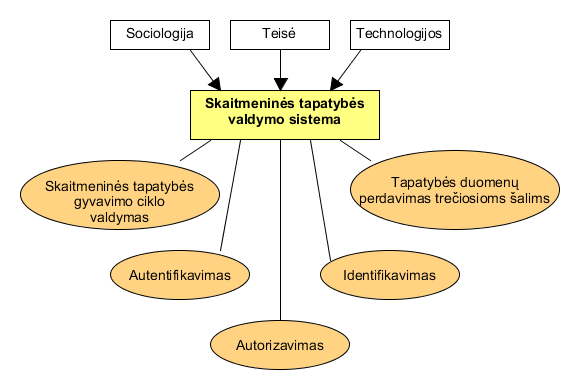
\includegraphics[scale=0.8]{img/IDMcontextAndUsecases}
    \caption{Skaitmeninių tapatybių valdymo sistemų kontekstas ir užduotys \cite{Glasser2009}}
\end{figure}

Paveiksle matomos disciplinos turi skirtingą poveikį tapatybių valdymo sistemoms. 
Sociologija padeda apibrėžti tapatybę ir jos atitikmenį skaitmeninėje erdvėje, teisės mokslas nusako tapatybės duomenų naudojimo reikalavimus,
o esamos technologijos formuoja sistemos įgyvendinimo niuansus. Verta pastebėti, kad tapatybės valdymo sistema gali atlikti ne visas
diagramoje nurodomas funkcijas, o tik dalį iš jų. Taip pat, 1-ame paveiksle bei visame darbe naudojamos skaitmeninės tapatybės valdymo sąvokos,
tokios kaip \textit{identifikavimas}, \textit{autentifikavimas} ar \textit{autorizavimas} neretai suprantamos skirtingai, o tai sukelia
vieningos terminologijos trūkumą ir dėl jo kylančius neaiškumus \cite{Glasser2009}. Dėl to skyriuje
\enquote{Sąvokų apibrėžimai} pateikiami darbe dažniausiai naudojamų terminų aiškinimai.

Esamų tapatybių valdymo sistemų architektūros bei veikimo principai yra skirtingi -  S. Clauß ir M.Köhntopp savo tyrime pastebi,
kad nėra vieningo standarto identiteto
valdymo sistemoms \cite{Claus2001}. Tolesniuose skyriuose, apžvelgus naudotojų bei paslaugų tiekėjų reikalavimus
tapatybės valdymo sistemoms, pateikiamos skirtingos technologijos
bei sprendimai, naudojami identiteto valdymui internete, jų privalumai bei trūkumai.

\subsection{Skaitmeninės tapatybės valdymo sistemų charakteristikos}

Skaitmeninės tapatybės valdymas yra plati sritis, kurią galima analizuoti iš skirtingų pusių.
Šiame darbe į skaitmeninių tapatybių valdymą žvelgta iš dviejų perspektyvų: naudotojo bei paslaugų tiekėjo \textcolor{red}{palikt tik naudotojo?}. Abi pusės,
priklausomai nuo savo poreikių, turi jiems aktualias identiteto valdymo sistemų savybes. Apžvelgiant skirtingas tapatybės valdymo sistemas,
didžiausias dėmėsys kreiptas į naudotojams bei paslaugų tiekėjams svarbiausius sistemų bruožus.

Tiek naudotojams, tiek paslaugų tiekėjams itin svarbus yra pasirinkto identiteto valdymo sprendimo patikimumas, t.y., asmens duomenų saugumo užtikrinimas.
Naudotojai nenori savo asmens duomenų nutekėjimo (angl. \textit{data leakage}) internete, tuo tarpu paslaugų tiekėjai negali rizikuoti prarasti naudotojų pasitikėjimo
jų paslauga pasirinkus nesaugų tapatybės valdymo sprendimą. Be patikimumo, naudotojams bei paslaugų tiekėjams aktualios ir 
kitos skaitmeninio identiteto sistemų savybės. Žemiau pateikiami pagrindiniai abiejų pusių poreikiai.
\\

\chapter{\textbf{Naudotojams svarbūs tapatybės valdymo sistemų bruožai:}}

\begin{itemize}
    \item identifikatorių bei slaptažodžių kiekis. Naudotojui vidutiniškai turint 25 paskyras, reikalaujančias slaptažodžių \cite{Florencio2007} bei naudojant
    nuo 2 iki 12-os el. paštų \cite{Gross2007}, jis tampa priverstas prisiminti vis daugiau identifikatorių. Atsimintinų autentifikavimo duomenų kiekiui
    augant, naudotojai yra linkę aukoti saugumą dėl patogumo ir naudoti panašius
    slaptažodžius skirtingose sistemose \cite{Pashalidis2003, Samar1999};
    \item asmens duomenų kontrolė. Pasak Nyderlanduose atliktų tyrimų, naudotojai jaučia, kad nekontroliuoja savo asmens duomenų internete \cite{Baars2016}. Dėl to
    naudotojai pradeda nepasitikėti taikomųjų programų kūrėjais, nes jie pilnai nežino, kokia informacija apie juos kaupiama ir kokioms
    sistemoms ji perduodama;
    \item patogumas (angl. \textit{usability}). Naudotojams skaitmeninės tapatybės valdymas dažnai yra tik pašalinis mechanizmas, reikalingas
    norint pasiekti paslaugą \cite{Dhamija2008}. Dėl šios priežasties sistemos naudojimosi patogumas yra svarbus - kuo tapatybės valdymas yra labiau integruotas
    su asmens jau naudojamomis sistemomis ir kuo mažiau jis reikalauja papildomo naudotojo įsitraukimo, tuo labiau naudotojas bus linkęs pasirinkti šį identiteto valdymo sprendimą.
\end{itemize}

\chapter{\textbf{Paslaugų tiekėjams aktualios tapatybės valdymo sistemų savybės:}}

\begin{itemize}
    \item kaštai, skirti tapatybės valdymui. Priklausomai nuo pasirinkto sprendimo,
    paslaugų tiekėjui gali tekti skirti daug arba mažai resursų (programuotojų, laiko, investavimo į technologijas)
    naudotojų tapatybės valdymo veiksmams užtikrinti;
    \item naudotojo patirties kontrolė (angl. \textit{user experience control}). Paslaugų tiekėjai siekia užtikrinti teigiamą
    naudotojų patirtį dėl geresnio naudojamumo, privatumo ir saugumo \cite{Dhamija2008}, o tapatybės valdymo sistemos veikimo primesti sprendimai (pvz. nukreipimai į kitą tinklalapį) gali daryti
    tam įtaką.
\end{itemize}

\subsection{Esamos skaitmeninių tapatybių valdymo sistemos}

Skirtingos tapatybių valdymo sistemos yra pagrįstos skirtingomis architektūromis, kurios įgalina
konkrečios sistemos veikimą. Šiame skyriuje apžvelgiami 3-ys dažniausiai naudojami tapatybių valdymo sistemų
modeliai bei pateikiami jų įgyvendinimo pavyzdžiai.

\subsubsection{Izoliuotas tapatybių valdymas}

\subsubsubsection*{Modelis}

Izoliuotame modelyje paslaugų tiekėjas yra ir tapatybės tiekėjas, nes visos su tapatybės valdymu
susijusios operacijos yra atliekamos vieno serverio. Tapatybės duomenų saugojimas, autentifikavimas
ir autorizavimas yra įgyvendinti paties paslaugų tiekėjo \cite{Cao2010} Kiekvienas naudotojas turi atskirus identifikatorius
kiekvienam paslaugų tiekėjui. Modelis grafiškai pavaizduotas žemiau esančiame paveiksle:

\begin{figure}[H]
    \centering
    \includegraphics[scale=0.65]{img/IsolatedModel}
    \caption{Izoliuotas skaitmeninės tapatybės valdymas \cite{Cao2010}}
\end{figure}

Pagal izoliuotą modelį, naudotojas turi savo paskyrą kiekvieno jam aktualaus paslaugų tiekėjo sistemoje. Kiekvieną kartą autentifikuojat ar autorizuojant
naudotoją, tai atlieka pats paslaugų tiekėjas, bendraudamas tiesiogiai su naudotoju (jo naršykle). Naudotojui prisijungus prie vieno tinklalapio ir gavus
prieigos raktą, jis gali toliau naudotis tinklalapiu, tačiau prireikus pasinaudoti kitu paslaugų tiekėju, tapatybės atpažinimo veiksmai (autentifikavimas, autorizavimas)
turės būti atlikti iš naujo su šiuo paslaugų tiekėju.

Šis modelis yra gana paprastas paslaugų tiekėjams, tačiau greitai tampa
nebekontroliuojamu naudotojams \cite{Josang2005}. Jis verčia naudotojus turėti daug paskyrų, identifikatorių bei slaptažodžių.
Tie patys tapatybės atpažinimo veiksmai (pvz. autentifikavimas) atliekamas iš naujo su kiekviena reikalinga paslauga. Naudotojui
sunku kontroliuoti savo asmens duomenis, nes jis juos patiki visiems paslaugų tiekėjams, kuriais naudojasi - tai apsunkina 
priežiūrą, kur kokie duomenys perduoti bei asmens duomenų atnaujinimą, kuris turi būti atliekamas su kiekvienu paslaugos tiekėju atskirai.

\textcolor{red}{jei reik, pastraipa paslaugų tiekėjo bruožams}.

\subsubsubsection*{Realizacijos}

Kadangi šis naudotojų autentifikavimo bei autorizavimo modelis naudojamas seniausiai,
yra gana nemažai jį įgyvendinusių taikomųjų programų. Lietuvoje šį modelį naudoja
\enquote{Tiketa}, \enquote{Bilietai.lt}, \enquote{Pigu.lt},
\enquote{Varle.lt}, pasaulyje - \enquote{Booking.com}, \enquote{Skycop}, \enquote{AirBnB} bei kitos platformos. Verta
pastebėti, kad dalis iš jų jau remiasi ne tik savo tapatybės valdymo, bet jau turi į savo sistemas integravę ir papildomų autentifikavimo būdų
(pvz. prisijungimą per \enquote{Facebook} ar \enquote{Google}).

Realizacijų technologiniai sprendimai dažniausiai nėra viešai prieinami.
Šiame modelyje kiekvienas paslaugų tiekėjas yra ir tapatybės tiekėjas, tad nereikia
specialaus protokolo, kuriuo duomenimis apsikeistų šios dvi esybės - visa tai pats nusprendžia
ir įgyvendina paslaugų tiekėjas.

\subsubsection{Centralizuotas tapatybių valdymas}

\subsubsubsection*{Modelis}
Centralizuotame skaitmeninių tapatybių valdyme egzistuoja vienas naudotojo identifikatorius,
naudojamas visų paslaugų tiekėjų \cite{Josang2005}. Paslaugų tiekėjo ir tapatybės tiekėjo funkcijos tampa atskirtos - 
tapatybės tiekėjas rūpinasi naudotojo identiteto valdymu, o paslaugų tiekėjas koncentruojasi į savo paslaugos tobulinimą.
Naudotojui šiame modelyje užtenka vieno identifikatoriaus ir slaptažodžio, su kuriais jis gali prisijungti prie visų to paties
paslaugų tiekėjo paslaugų. Šis modelis iliustruotas ~\ref{fig:isolatedModel}-iame paveiksle.

Iš naudotojo perspektyvos, šis modelis yra patogesnis nei izoliuotas. Naudotojui pakanka turėti vieną identifikatorių,
kuris bus tinkamas visoms paslaugoms. Priklausomai nuo realizacijos, naudotojui gali tekti iš naujo prisijungti prie kiekvienos
paslaugos arba vieną kartą prisijungti prie betkurios iš paslaugų ir tapti autentifikuotu visose kitose paslaugose \cite{Josang2005}. Naudotojo asmens
duomenų kontrolė yra geresnė nei izoliuotame skaitmeninės tapatybės valdyme, nes naudotojas asmens duomenis patiki mažesniam kiekiui esybių
(vietoj kiekvienos paslaugos, kiekvienam paslaugų tiekėjui).

Pagrindinis šio modelio trūkumas yra tas, kad jis galimas naudoti tik vieno paslaugų tiekėjo srityje (angl. \textit{scope}). Tai palieka laisvės paslaugų tiekėjui tapatybės valdymo sistemos
realizavimui (tai gali būti centralizuota platforma įmonės ribose), tačiau naudotojas negali turimo identifikatoriaus
naudoti kito paslaugų tiekėjo sistemose.

\begin{figure}[H]
    \centering
    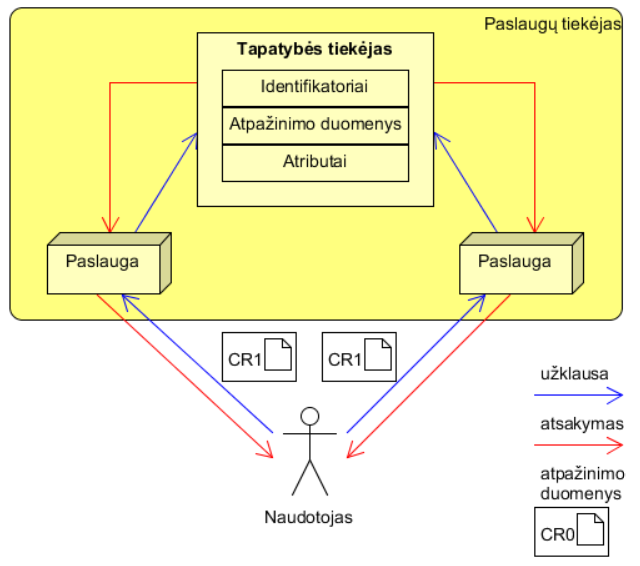
\includegraphics[scale=0.8]{img/centralizedModel}
    \caption{Centralizuotas skaitmeninės tapatybės valdymas \cite{Cao2010}}
    \label{fig:isolatedModel}
\end{figure}

\textcolor{red}{jei reik, pastraipa paslaugų tiekėjo bruožams}.

\subsubsubsection*{Realizacijos}

Centralizuotas modelis tinkamas naudoti vieno paslaugų tiekėjo ribose \cite{Josang2005}. Vienas iš pavyzdžių - 
\enquote{Atlassian} įmonės paslaugos. Naudotojui pakanka turėti vieną \enquote{Atlassian} paskyrą ir jis gali naudotis
skirtingais šio paslaugų tiekėjo produktais, tokiais kaip \enquote{Jira}, \enquote{Confluence}, \enquote{Bitbucket} bei kitais. \enquote{Atlassian}
turi ir vienkartinio prisijungimo sąlygas - paslaugas galima sukonfigūruoti taip, kad prisijungus prie vienos iš jų,
naudotojas automatiškai tampa prisijungęs ir prie kitų paslaugų.

Realizacijų naudojamos technologijos nėra viešai skelbiamos. Kadangi centralizuotame modelyje paslaugų tiekėjas
pats įgyvendina tapatybės tiekėjo modulį, jis pats apsprendžia bendravimą tarp tapatybės ir paslaugų tiekėjo. Priklausomai
nuo skirtingų paslaugų dydžio ir reikmių, šis bendravimas su tapatybės tiekėju gali svyruoti nuo centralizuotos duomenų bazės
naudotojų duomenims iki
paskirstytame tapatybės valdyme naudojamų technologijų (SAML, OpenID).

\subsubsection{Jungtinis tapatybių valdymas}

\subsubsubsection*{Modelis}

Centralizuotas modelis reikalauja visų naudotojų būti tame pačiame domene, tačiau naudotojams reikia
paslaugų ir iš kitų domenų \cite{Cao2010}. Jungtinis (angl. \textit{federated}) tapatybių valdymas yra aibė technologijų
ir procesų, kurie leidžia sistemoms dalintis tapatybės informacija ir deleguoti tapatybės valdymo užduotis
tarp skirtingų paslaugų tiekėjų \cite{Maler2008}. Šis tapatybių valdymo modelis įgalina naudotojus turėti vieną
identifikatorių, kurį gali naudoti skirtingų paslaugų tiekėjų tinklalapiuose. Žemiau pateikiama schema, nusakanti
šio modelio architektūrą:

\begin{figure}[H]
    \centering
    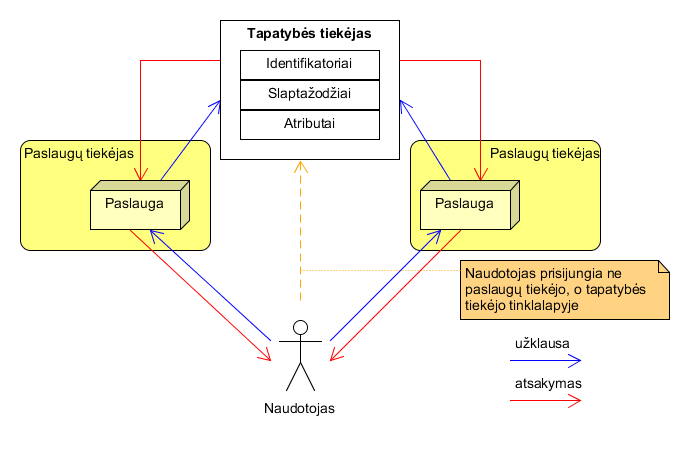
\includegraphics[scale=0.75]{img/federatedModel}
    \caption{Jungtinis skaitmeninės tapatybės valdymas \cite{Cao2010}}
    \label{fig:federatedModel}
\end{figure}

Jungtiniame tapatybės valdyme tapatybės tiekėjas yra atskira sistema, su kuria turi integruotis paslaugų tiekėjas. Tapatybės
duomenys bei su tapatybe susiję veiksmai (autentifikavimas, autorizavimas) yra deleguojami šiai sistemai. Naudotojas turi vieną identifikatorių,
su kuriuo prisijungia tiesiogiai tapatybės tiekėjo puslapyje. Prisijungus šioje sistemoje, naudotojas tampa
autentifikuotas visose paslaugose, kurios palaiko šį tapatybės tiekėją \cite{Maler2008}.

Šis tapatybių valdymo modelis yra gana patogus naudotojams. Jiems užtenka turėti vieną identifikatorių, su kuriuo
gali prisijungti prie tinklalapių iš skirtingų paslaugų tiekėjų. Asmens duomenų saugumas priklauso nuo
bendravimo tarp paslaugų bei tapatybės tiekėjų, o šiame modelyje jis sudėtingesnis nei izoliuotame ar centralizuotame
tapatybių valdyme, nes jungtinis valdymas paremtas tarpdomeniniu bendravimu \cite{Maler2008}. Naudotojo duomenų kontrolė jungtiniame 
modelyje turi tiek privalumų, tiek trūkumų. Viena vertus, naudotojas savo asmens duomenis suteikia mažesniam kiekiui sistemų (tik tapatybės tiekėjams,
vietoj visų paslaugų tiekėjų). Tačiau taip paslaugų tiekėjas tampa vieninteliu nesekmės tašku (angl. \textit{single point of failure}) - programišiams įsilaužus
į tapatybės tiekėjo sistemą, asmens paskyros visose paslaugose tampa prieinamos \cite{Pashalidis2003}. Taip pat, naudotojui gali būti sunku kontroliuoti
savo duomenų sklaidą tarp tapatybės tiekėjo ir skirtingų paslaugų, ką rodo ir \textit{Cambridge Analytica} incidentas \cite{CambridgeAnalytica}.

\textcolor{red}{jei reik, pastraipa paslaugų tiekėjo bruožams}.

\subsubsubsection*{Realizacijos}

\textcolor{red}{to be added}

\subsection{Tapatybių valdymo sistemų palyginimas}

% Please add the following required packages to your document preamble:
% \usepackage{multirow}
% \usepackage{graphicx}
\begin{table}[h]
    \centering
    \caption{My caption}
    \label{my-label}
    \resizebox{\textwidth}{!}{%
    \begin{tabular}{|l|l|l|l|l|l|}
    \hline
    \multicolumn{1}{|c|}{\multirow{2}{*}{Modelis}} & \multicolumn{1}{c|}{\multirow{2}{*}{\begin{tabular}[c]{@{}c@{}}Identifikatorių\\ kiekis\end{tabular}}} & \multicolumn{3}{c|}{Patogumas} & \multicolumn{1}{c|}{\multirow{2}{*}{\begin{tabular}[c]{@{}c@{}}Asmens duomenų\\ kontrolė\end{tabular}}} \\ \cline{3-5}
    \multicolumn{1}{|c|}{} & \multicolumn{1}{c|}{} & \multicolumn{1}{c|}{\begin{tabular}[c]{@{}c@{}}Prisijungimų\\ kiekis\end{tabular}} & \multicolumn{1}{c|}{\begin{tabular}[c]{@{}c@{}}Papildoma programinė\\ įranga\end{tabular}} & \multicolumn{1}{c|}{Naudotojo patirtis} & \multicolumn{1}{c|}{} \\ \hline
    Izoliuotas &  &  &  &  &  \\ \hline
    Centralizuotas &  &  &  &  &  \\ \hline
    Jungtinis &  &  &  &  &  \\ \hline
    \end{tabular}%
    }
    \end{table}
\section{Blokų grandinės technologija} \label{section:blockchainOverview}

Blokų grandinė - tai vieno su kitu susijusių blokų grandinė, kurios blokuose saugomi
nekeičiami įrašai \cite{SatoshiNakamoto}. Šią technologiją galima apibūdinti kaip daugybę paskirstytų nekintamų skaitmeninių įrašų 
(angl. \textit{immutable distributed ledger}), tarpusavyje susietų taikant kriptografiją (blokų grandinės pavyzdys pateikiamas\hypertarget{fig:blockchain}{~\ref{fig:blockchain}} paveiksle). Technologija geriausiai žinoma dėl jos panaudojimo \enquote{Bitcoin} kriptovaliutoje.
Šiame skyriuje apžvelgiami pagrindiniai blokų grandinės techniniai aspektai, savybės bei galimi skirtingi variantai.

\begin{figure}[H]
    \centering
    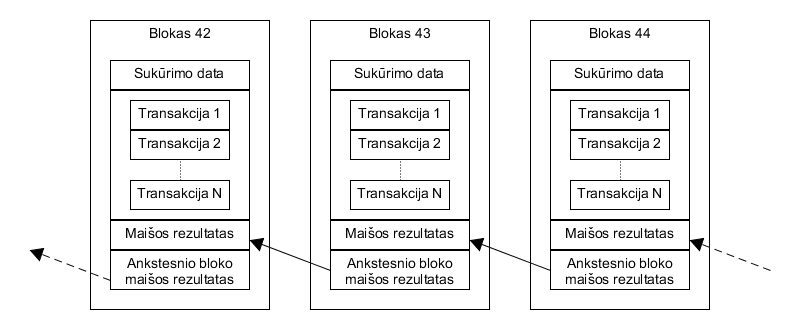
\includegraphics[scale=0.6]{img/blockchain}
    \caption{Supaprastintas blokų grandinės modelis}
    \label{fig:blockchain}
\end{figure}

\subsection{Nekintamumas}

Blokų grandinėje kiekvienas blokas yra sudarytas iš šių dalių:

\begin{itemize}
    \item transakcijų. Kiekviena transakcija yra duomenys, kuriuos norima saugoti blokų grandinėje. Šie duomenys gali būti bet kokia vertinga informacija:
    pervesti pinigai, programinis kodas, skaitmeninės tapatybės atributai ar kt. Kiekviena transakcija yra pasirašoma
    kūrėjo privačiu raktu. Vienas blokas gali turėti vieną arba daugiau transakcijų;
    \item bloko kriptografinės maišos funkcijos rezultato (angl. \textit{hash});
    \item ankstesnio (tėvinio) bloko kriptografinės maišos funkcijos rezultato;
    \item bloko sukūrimo laiko. Blokai grandinėje saugomi chronologiškai;
    \item kitų metaduomenų (pvz. bloko eilės numerio, blokų grandinės versijos, \textit{nonce} darbo įrodymui).
\end{itemize}

Kiekvieno bloko maišos funkcijos rezultatas priklauso nuo jo transakcijų, prieš tai buvusio bloko maišos rezultato ir bloko metaduomenų.
Jeigu betkurio bloko duomenys būtų pakeisti, tuomet maišos funkcija sugeneruotų kitokį maišos rezultatą ir būtų lengva patikrinti, kad
naujai perskaičiuotas maišos rezultatas nesutampa su bloke esančiu rezultatu. Taip pat, kadangi kiekvienas blokas
priklauso nuo prieš tai buvusio bloko, net ir pakeitus vieną iš pirmųjų blokų, pakeitimas būtų pastebimas pridedant naujus blokus ir būtų galima suprasti,
kad turima blokų grandinės versija yra nevalidi (žr.\hypertarget{fig:blockchainNotIntact}{~\ref{fig:blockchainNotIntact}} pav.). Tokiu būdu kiekvienas blokų grandinės blokas patvirtina prieš tai
buvusio bloko integralumą, taip pasiekiant blokų grandinės nekintamumą (angl. \textit{immutability}),
nes perrašyti įrašus blokuose nepastebėtam labai sunku \cite{SatoshiNakamoto}.

\begin{figure}[H]
    \centering
    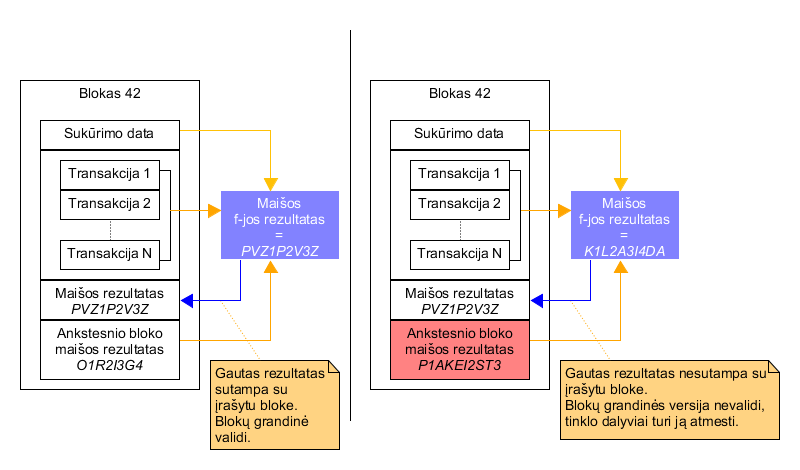
\includegraphics[scale=0.6]{img/blokchainNotIntact}
    \caption{Bloko grandinėje validavimas}
    \label{fig:blockchainNotIntact}
\end{figure}

\subsection{Decentralizuotumas}

Blokų grandinės sistema yra decentralizuota - nėra vieno centrinio serverio, kuris vienas turėtų visą blokų grandinę.
Sistemą sudaro daugybė blokų grandinės mazgų (angl. \textit{node}), kurie turi visą blokų grandinės kopiją. Šie mazgai
yra atsakingi už naujų transakcijų validavimą, blokų su transakcijomis kūrimą, sukurtų blokų priėmimą į blokų grandinę ir pranešimus kitiems mazgams apie naują į grandinę priimtą
bloką \cite{Antonopoulos2016}. Kiekvienas mazgas yra susietas su keletu kitu mazgų. Mazgas, kuris nori pridėti naują bloką (vadinamas \textit{kasėju}), praneša apie jį
kitiems mazgams, jie savo ruožtu žinią perduoda kitiems mazgams ir taip ilgainiui kiekvienas mazgas tinkle turi naujausią blokų grandinės versiją.

Kadangi nėra centrinės institucijos, kuri nuspręstų, ar siūlomas blokas yra tinkamas priimti į grandinę, sprendimą bendrai turi priimti
visi tinklo dalyviai. Egzistuoja skirtingos taisyklės, vadinamos konsensuso strategijomis (plačiau apie juos\hypertarget{blockchain:consensus}{~\ref{blockchain:consensus}} skyrelyje), kuriomis
remdamiesi tinklo mazgai nusprendžia, ar pasiūlytas blokas yra validus. Šios taisyklės apibrėžia, kaip tinklo dalyviai turi įrodyti bloko validumą jį siūlydami į grandinę
bei kaip patikrinti kito dalyvio pasiūlyto bloko validumą.

\subsection{Tipai}

Priklausomai nuo tinklo dalyviams suteikiamų blokų grandinės skaitymo ir rašymo teisių,
išskiriami trys pagrindiniai blokų grandinės tipai: vieša, konsorciumo bei privati.  Tipų skirtumai pateikiami\hypertarget{tab:blockchainComparison}{~\ref{tab:blockchainComparison}} lentelėje.

% \caption{Viešos, konsorciumo ir privačios blokų grandinės palyginimas \cite{Zheng2017}}
% \label{tab:blockchainComparison}
% Table generated by Excel2LaTeX from sheet 'BlockchainComparison'
\begin{table}[htbp]
    \centering
    \caption{Viešos, konsorciumo ir privačios blokų grandinės palyginimas \cite{Zheng2017}}
      \begin{tabular}{|p{8.11em}|l|p{10.22em}|p{6.055em}|}
      \hline
      \multicolumn{1}{|r|}{} & \textbf{Vieša} & \textbf{Konsorciumo} & \textbf{Privati} \bigstrut\\
      \hline
      \textbf{Konsensuso nustatymas} & Visi kasėjai & Išrinkti tinklo dalyviai & Viena organizacija \bigstrut\\
      \hline
      \textbf{Skaitymo teisės} & Viešos & Gali būti viešos ar apribotos & Gali būti viešos ar apribotos \bigstrut\\
      \hline
      \textbf{Centralizuotumas} & Nėra & Dalinis & Yra \bigstrut\\
      \hline
      \textbf{Efektyvumas} & Mažas & Didelis & Didelis \bigstrut\\
      \hline
      \end{tabular}%
    \label{tab:blockchainComparison}%
  \end{table}%
  

Kadangi vieša blokų grandinė yra atvira visam pasauliui, visiems matomos ir joje išsaugotos transakcijos. Tai sudaro puikias salygas įrašų
auditui, tačiau sumažina naudotojų privatumą. Siekiant išlaikyti tam tikrą privatumo lygį, viešoje grandinėje matomi tik transakcijas atlikusių 
asmenų vieši raktai \cite{SatoshiNakamoto}. Viešų blokų grandinių pavyzdžiai: \enquote{Bitcoin}, \enquote{Ethereum} kriptovaliutų blokų grandinės.

Privačios bei konsorciumo blokų grandinės yra tik dalinai decentralizuotos - jose blokų validavimą ir priėmimą į grandinę atlieka vienas
ar dalis tinklo dalyvių. Šios grandinės privalumai: visi validuotojai yra žinomi, grandinės efektyvesnės dėl greičiau priimamų blokų, apribotos blokų skaitymo teisės suteikia didesnį
privatumo lygį, o iškilus poreikiui, tinklo dalyviai gali pakeisti ar atšaukti įvykusias transakcijas \cite{Buterin2015}. Konsorciumo ir privačios blokų grandinės labiau tinkamos įmonių vidiniam (ar jungtiniam,
pvz. tarp kelių finansinių institucijų) naudojimui. Blokų grandinių karkasų sprendimus įmonėms siūlo \enquote{IBM}, \enquote{Microsoft}, \enquote{Amazon} \cite{Zheng2017}.

\subsection{Konsensuso strategijos} \label{blockchain:consensus}

Kadangi blokų grandinės sistema yra decentralizuota, nėra centrinės institucijos, kuri nuspręstų, ar naujai siūlomas pridėti į grandinę blokas
yra validus (be transakcijų su falsifikuotais duomenimis). Todėl blokų grandinės tinkle taikoma konsensuso strategija,
pagal kurią nusprendžiama, ar pridėti naują bloką į grandinę. Apžvelgiamos trys dažnai naudojamos strategijos: darbo, įtakos bei autoriteto įrodymo.

\subsubsection{Darbo įrodymo strategija}

Darbo įrodymo konsensuso strategija remiasi principu, kad daug pastangų ir resursų į bloko validumo įrodymą įdėjęs tinklo
dalyvis nebus linkęs sukčiauti. Šioje strategijoje tinklo dalyvis, norėdamas pridėti bloką į blokų grandinę, turi išspręsti laikui ir resursams
imlų matematinį
uždavinį (užsiima \textit{bloko kasimu}). Pirmas uždavinio reikšmę radęs tinklo dalyvis praneša apie ją kitiems, kurie turi patvirtinti,
ar ši reikšmė teisinga. Jei tai patvirtinta, tinklo dalyviai patikrina, ar naujojo bloko transakcijos yra validžios. Jeigu jos validžios,
blokas pridedamas į grandinę \cite{Zheng2017}.

Darbo įrodymo matematinis uždavinys dažniausiai būna paremtas kriptografine maišos funkcija, kurios rezultatą lengvą validuoti,
tačiau duomenis, sugeneravusius šį rezultatą, sunku surasti. Uždavinio tikslas - surasti šiuos duomenis. Tinklo dalyviai eikvoja didžiulius
kiekius elektros energijos ir laiko,
nes radimas būna paremtas duomenų perrinkimu (angl. \textit{brute force}). Dėl šios priežasties rezultato ieškantiems \textit{kasėjams}
 neretai būna įvesta paskatinimo sistema, kuri teisingą reikšmę radusį
\textit{kasėją} apdovanoja piniginiu atlygiu \cite{SatoshiNakamoto}. 

Kadangi blokų grandinės tinklas yra decentralizuotas, įmanoma situacija, kad labai panašiu metu į grandinę skirtingų mazgų pridėti du validūs blokai.
Taip dalis tinklo dalyvių gaus vieną mazgą, o dalis - kitą, o abu jie bus susieti su tuo pačiu prieš tai buvusiu bloku.
Tokiu atveju, taikoma ilgiausios grandinės taisyklė (žr.\hypertarget{fig:blockchainLongestRule}{~\ref{fig:blockchainLongestRule}} pav.). Mazgai dirba prie pirmiau gauto bloko,
tačiau išsaugo kitą gautą bloką kaip šaką. Po to, kai bus gautas dar vienas blokas, jis bus susietas tik su viena iš šakų - taip ši šaka taps ilgesnė. Tuomet
ilgesnė šaka paskelbiama aktyviąja grandine, visi su trumpesniąja šaka dirbę mazgai turi pereiti prie aktyviosios grandinės, o atmesto bloko (vadinamo \textit{bloku-našlaičiu}) transakcijos
grąžinamos į bendrą transakcijų sankaupą (angl. \textit{transaction pool}) \cite{SatoshiNakamoto}.
Realiuose blokų grandinės taikymuose, dažnai laukiama keleto iš eilės einančių naujų blokų, kol \textit{blokas-našlaitis}
yra atmetamas. Pavyzdžiui,
\enquote{Bitcoin} blokų grandinėje tik sulaukus apytiksliai 6 blokų iš eilės \textit{blokas-našlaitis} gali būti atmestas\cite{Zheng2017}.

\begin{figure}[H]
    \centering
    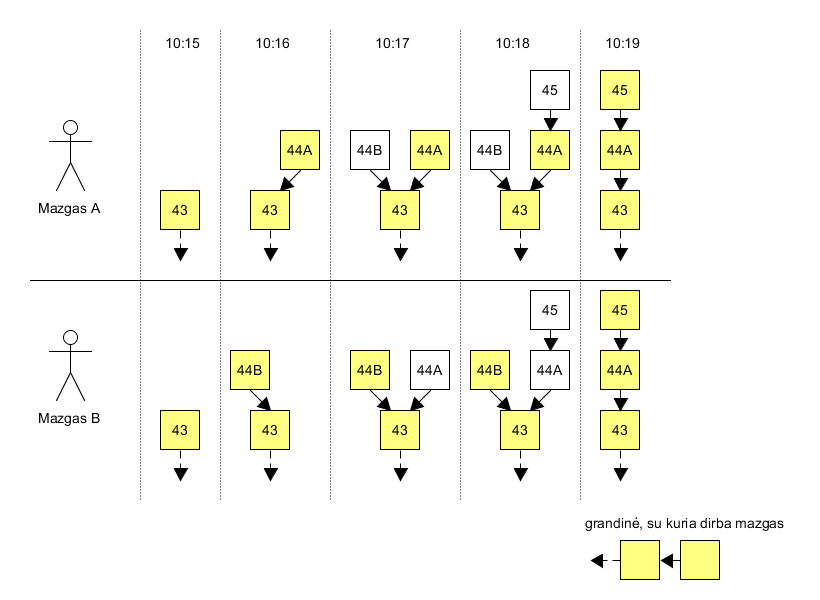
\includegraphics[scale=0.6]{img/blockchainLongestRule}
    \caption{Ilgiausios grandinės taisyklės taikymas}
    \label{fig:blockchainLongestRule}
\end{figure}

Pagrindinis šios konsensuso strategijos privalumas yra tas, kad dideli kasimo kaštai gali atgrasyti programišius nuo potencialių atakų. Tačiau,
taip veltui išeikvojama daugybė elektros energijos - skaičiuojama, kad kasimas \enquote{Bitcoin} ir \enquote{Ethereum} blokų grandinėms kartu sudėjus per dieną
sueikvoja elektros energijos, kurios vertė yra apie 1 milijoną dolerių \cite{Ethereum}. Taip pat, dėl ilgo uždavinio sprendimo laiko vieno bloko priėmimas į grandinę
gali užtrukti - Bitcoin blokų grandinėje tai užima apie 10 minučių \cite{Zheng2017}.

\subsubsection{Turto įrodymo strategija}

Turto įrodymo konsensuso strategija remiasi principu, kad daug blokų grandinės turto turintis kasėjas
bus sąžiningas, nes išaiškinus jo nesąžiningumą jis rizikuoja prarasti savo turimą turtą \cite{Baars2016}. Šis algoritmas patiki sprendimą priimti
tiems tinklo dalyviams, kurie įrodo kad turi daugiausia turto (pvz. blokų grandinės kriptovaliutos). Remiantis tik šia savybe, tokia strategija gali pasirodyti kaip ne itin sąžininga,
nes turtingiausias tinklo dalyvis gali būti vienvaldžiu sprendimų priėmėju. Dėl to blokų grandinės tinklai neretai taiko patobulintus šios strategijos
variantus: \enquote{Peercoin} papildomai vertina turto amžių, \enquote{Blackcoin} kitą patvirtintoją paskiria pagal atsitiktinę funkciją, kuri atsižvelgia ir į turimą turtą \cite{Zheng2017}.

Ši strategija leidžia nebeeikvoti didžiulių elektros kiekių, skirtingai nei darbo įrodymo strategija \cite{Ethereum}. Algoritmo efektyvumas
taip pat sutaupo laiko ir blokai būna greičiau patvirtinami ir pridedami į grandinę. Tačiau, dėl praktiškai nulinių bloko \textit{kasimo} sąnaudų,
galimos dažnesnės tinklo atakos \cite{Zheng2017}. 

\subsubsection{Autoriteto įrodymo strategija}

Autoriteto įrodymo strategija remiasi keleto tinklo dalyvių, kuriems suteikta teisė validuoti naujus blokus, priimamais sprendimais. Ši strategija nebėra tinkama visiškai
decentralizuotai blokų grandinei, kurioje būtinas pilnas pasitikėjimo padalinimas \cite{ProofOfAuthority}. Tačiau ši strategija tinkama privačioms
ar konsorciumo blokų grandinėms.

Šis konsensuso mechanizmas remiasi iš anksto išrinktais tinklo dalyviais, kurie bus atsakingi už blokų validavimą. Kiekvieną kartą pridedant naują
bloką į grandinę, vienas iš išrinktų validuotojų patvirtins arba atmes pasiūlytą bloką. Siekiant sumažinti galimą kenksmingų patvirtintojų žalą,
įvedamos taisyklės, neleidžiančios tam pačiam validuotojui patvirtinti keleto blokų iš eilės \cite{ProofOfAuthority}.

Autoriteto įrodymo strategijoje validuotojams svarbu išlaikyti gerą reputaciją - susigadinus ją, validuotojas gali būti pašalintas iš tinklo. Šis konsensuso mechanizmas
leidžia greitai ir su itin mažais ištekliais pridėti blokus, tačiau nėra tinkamas pilnai decentralizuotoms blokų grandinėms. Šią strategiją
taiko \enquote{Parity} blokų grandinė \cite{ProofOfAuthority}.

\subsection{Išmanieji kontraktai}

Išmanusis kontraktas (angl. \textit{smart contract}) - tai kompiuterizuotas transakcijos protokolas, kuris
išpildo kontrakto sąlygas, jei patenkinami numatyti kriterij \cite{Szabo1997}.
Išmanųjį kontraktą galima apibūdinti kaip tam tikras sąlygas (išreikštas kodu), kurios, patenkinus reikalavimus, bus įvykdytos automatiškai,
be trečiosios šalies priežiūros.

Idėja, pristatyta dar prieš 2000-uosius, šiais laikais yra įgyvendinama pasitelkiant blokų grandinę. Išmanusis kontraktas
į blokų grandinę yra patalpinamas kaip transakcija. Tuomet, dėl blokų grandinės viešumo, kodo logika būna atskleista ir kiekvienas norintis
gali įsitikinti, ar kontraktas veiks tinkamai. Taip pat, kadangi pats išmanusis kontraktas yra blokų grandinės transakcijoje, jis nebegali būti keičiamas.
Tai padidina naudotojų pasitikėjimą, nes jokia centrinė institucija negali
pakeisti kontrakto sąlygų. Tačiau, jei kode palikta defektų, jų nebebus galima ištaisyti.

Blokų grandinėje esančių išmaniųjų kontraktų kodas yra vykdomas automatiškai tinkle esančių kasėjų \cite{Zheng2017}.
Taip nebelieka vienintelio nesekmės taško situacijos, kai kodą vykdytų vienas centrinis serveris - išmaniojo kontrakto
kodas butų nebevykdomas tik tada, jei visi tinklo mazgai išeitų iš tinklo. Už tai, kad tinklo dalyviai naudoja savo kompiuterių
resursus išmaniųjų kontraktų kodui vykdyti, jiems dažniausiai suteikiamas piniginis paskatinimas.

Išmaniųjų kontraktų veikimo detalės priklauso nuo blokų grandinės, kurioje jie bus vykdomi.
Bene žinomiausia išmaniųjų kontraktų kūrimui pritaikyta platforma - \enquote{Ethereum}.
\hypertarget{section:ethereumIntro}{\ref{section:ethereumIntro}} skyrelyje apžvelgiamos pagrindinės išmaniųjų kontraktų
veikimo sąlygos.

\subsubsection{\enquote{Ethereum} išmanieji kontraktai} \label{section:ethereumIntro}

2015-aisias pradėjusi veikti \enquote{Ethereum} platforma pristatė blokų grandinę, kuri pritaikyta kurti būseną galinčius keisti
išmaniuosius kontraktus su išbaigta
(angl. \textit{turing complete}) programavimo kalba \cite{EthereumWhitePaper}. \enquote{Ethereum} kontraktai vykdomi tinklo
dalyvių, \enquote{Ethereum} virtualiosios mašinos pagalba.  \enquote{Ethereum} virtualioji mašina gali būti suprantama kaip didelis decentralizuotas
kompiuteris, saugantis milijonus objektų, vadinamų paskyromis, kurie turi galimybę turėti savo duomenis,
vykdyti kodą bei bendrauti tarpusavyje \cite{Ethereum}.

\enquote{Ethereum} platforma turi paskyras, kuriomis naudojantis, galima kurti transakcijas bei kviesti išmaniųjų
kontraktų funkcijas. Paskyros identifikuojamos pagal unikalų adresą. \enquote{Ethereum} egzistuoja dviejų tipų paskyros \cite{Ethereum}:

\begin{enumerate}
    \item išorinės paskyros (angl. \textit{externally owned accounts}). Jos savininkų valdomos privačiais raktais ir turi eterio
    balansą;
    \item kontraktų paskyros (angl. \textit{contract accounts}). Šios paskyros be balanso turi kodą bei būseną, kuri gali keistis,
    jei įvykdomos kode aprašytos sąlygos. Kontraktų paskyros yra valdomos kontrakto kodo.
\end{enumerate}

Skatinant tinklo dalyvius vykdyti kontraktų kodą, jiems už šį darbą skiriama piniginė premija - eterio kriptovaliuta. Kiek eterio
bus skiriama, priklauso nuo vykdomo kodo sudėtingumo ir jam reikalingų resursų. Dėl to kiekviena kodo operacija \enquote{Ethereum} platformoje
yra įvertinama kuro (angl. \textit{gas}) kiekiu, kuris nurodo sąlyginę kainą. Kuro sistema padeda apsisaugoti nuo begalinių ciklų vykdymų - jei vykdant
funkciją baigiasi kuras, vykdymas nutraukiamas, o kuras kvietėjui nėra grąžinamas \cite{EthereumWhitePaper}.\\
Skiriamos dviejų tipų funkcijos: rašymo bei skaitymo. Skaitymo funkcijų kvietimas yra nemokamas - jos tik grąžina
esamus kontrakto duomenis. Rašymo funkcijos yra mokamos, nes jos keičia kontrakto būseną. Jų vykdymo metu turi būti sukurta transakcija,
kurią patvirtins \enquote{Ethereum} blokų grandinės dalyviai. Kuo didesnis duomenų kiekis bus išsaugotas būsenoje, tuo brangesnė bus operacija.

Funkcijos kvietimą apmoka kvietėjas. Dėl šios priežasties kvietėjas savo paskyroje turi turėti eterio, iš kurio galės padengti
kviečiamos funkcijos išlaidas. Norint neversti kvietėjo apmokėti, kontrakto kodas kviečiamos funkcijos pabaigoje gali į kvietėjo paskyrą
pervesti jo išeikvotą eterį. Tolimesnėse \enquote{Ethereum} versijose svarstoma įdiegti funkcionalumą,
kuris standartizuotų būdą, leisiantį kontraktams patiems apmokėti iškviestų funkcijų išlaidas \cite{ContractPays}.

\subsection{Pavojai ir trūkumai} \label{blockchain:concerns}

Blokų grandinės technologija sukuria sąlygas decentralizuotai, nesuteikiant pasitikėjimo vienam ar keliems dalyviams, laikyti nekeičiamus duomenis.
Tai atveria įvairių galimybių finansų, daiktų interneto, reputacijos sistemų ar saugumo srityse \cite{Zheng2017}, tačiau ši technologija turi ir trūkumų,
kurių galimą poveikį būtina įvertinti prieš taikant šią technologiją konkrečioje sferoje. Pagrindinės grėsmės ir trūkumai aptariami šiame skyriuje.

\subsubsection{Daugumos ataka}

Viešose blokų grandinėse dauguma (>50\%) mazgų tinkle turi patvirtinti bloką, kad jis būtų priimtas į grandinę. Potencialus įsilaužėlis gali pateikti
falsifikuotą blokų grandinės bloką (pvz. su netikromis transakcijomis), tačiau kol jis neturi daugumos skaičiavimo galios tinkle, šis blokas bus
atmestas likusių dalyvių mazge (ir taps \textit{bloku-našlaičiu} taikant ilgiausios grandinės taisyklę). Tačiau, jeigu įsilaužėlis (ar keletas jų)
turi daugumą skaičiavimo galios, jis gali dirbti su falsifikuota blokų grandinės versija greičiau negu likę dalyviai tinkle ir taip ilgiausia grandine, prie kurios
pereis visi dalyviai, taps jo sukurta grandinė su falsifikuotais blokais \cite{Zheng2017}. Ši ataka nebuvo įgyvendinta prieš žinomiausias \enquote{Bitcoin} bei \enquote{Ethereum} blokų grandines, tačiau
buvo įvykdyta prieš \enquote{Verge} blokų grandinę \cite{Sedgwick2018}.

\subsubsection{Plečiamumas}

Blokų grandinės plečiamumas matuojamas pagal du kriterijus: transakcijų pralaidumą ir saugojimo reikalavimus mazgams. Transakcijų pralaidumas, kuris priklauso nuo to,
kaip greitai nauji blokai yra pridedami į blokų grandinę, susijęs su taikoma konsensuso strategija.
Kuo taikoma strategija leidžia greičiau priimti naują bloką, tuo greičiau transakcijos bus patvirtintos. \enquote{Bitcoin} kriptovaliutos blokų grandinėje, taikančioje darbo įrodymo konsensusą,
apdorojoma apie 7 transakcijas per sekundę \cite{Zheng2017}, kai \enquote{Tendermint} blokų grandinė, taikanti
atsparumo klaidoms konsensusą, teigia galinti apdoroti tūkstančius transakcijų per sekundę \cite{Tendermint2017}. Dėl darbo įrodymo strategijos neefektyvumo
blokų grandinės neretai tampa priverstos iškeisti ją į efektyvesnį konsensuso būdą - \enquote{Ethereum} blokų grandinė ketina pereiti prie turto įrodymu grįsto konsensuso \cite{Ethereum}.

Kita priežastis, dėl ko transakcijos tvirtinamos gana lėtai - blokai turi dydžio apribojimus. Dėl šių apribojimų, tik dalis susikaupusių transakcijų gali būti priimtos
į naują bloką, o likusios turi laukti, kol pateks į kitą bloką. Tam spręsti pasitelktos šalutinės blokų grandinės. Jos dalį bloko duomenų iškelia į šalutinę grandinę,
taip palikdamos daugiau vietos pagrindinės grandinės bloke. Tokį sprendimą priėmė \enquote{Bitcoin} blokų grandinė, į tinklą pristatydama \enquote{SegWit} protokolą, kuris iškelia skaitmeninių
parašų duomenis į atskirą grandinę \cite{Segwit}.

Visos blokų grandinės dydis taip pat gali sukelti plečiamumo problemų. Šiuo metu Bitcoin blokų grandinė užima per 100 gigabaitų \cite{Zheng2017}. Siekiant sumažinti blokų grandinės
(kurią turi kiekvienas mazgas tinkle) dydį,
siūlomi įvairūs sprendimai. Vienas variantas yra mazgams neturėti seniausių blokų grandinės dalių, o senus blokus su transakcijomis iškelti į atskirą duomenų bazę.
Kitas sprendimo būdas - pagrindinėje blokų grandinėje laikyti tik transakcijų maišos rezultatus, o pačius transakcijų duomenis
iškelti už grandinės ribų (angl. \textit{off-chain}) \cite{Lo2017}.

\subsubsection{Anonimiškumas}

Manoma, kad blokų grandinės išsaugo naudotojų privatumą dėl to, kad transakcijose atskleidžiamas tik naudotojų
viešas raktos vietoj tikrosios tapatybės \cite{Zheng2017}. Tačiau, tyrimai rodo, kad iš viešojo rakto galima
atsekti tikrąją naudotojo tapatybę \cite{Barcelo2007}. Taip pat, transakcijoje buvę duomenys (pvz. pervestas pinigų kiekis)
viešoje blokų grandinėje bus matomas visiems tinklo dalyviams.

Galimi skirtingi sprendimai didesniam anonimiškumui pasiekti. Pirmiausia, reikia atsižvelgti, ar negalima naudoti privačios blokų grandinės, kurioje
blokų skaitymo teisės būtų apribotos. Kitas variantas - blokų grandinėje saugoti užšifruotus duomenis, kurių skaitymui
reikia turėti dešifravimo raktą. Jeigu tai netinkama išeitis, tuomet transakcijas galima atlikti per tarpininką, kuris išskaidys vieną transakciją
į keletą, vykdomų su skirtingais viešaisiais raktais, ir taip bus sunkiau atsekti transakcijos autorių \cite{Zheng2017}.


\section{Blokų grandinės naudojimas skaitmeninės tapatybės valdyme} \label{section:BCusageinIDM}

Šiame skyriuje nagrinėjamas blokų grandinės technologijos panaudojimas tapatybės valdyme.
Tiriama, kaip blokų grandinės savybės gali padėti išspręsti egzistuojančias
naudotojų problemas, apžvelgiami technologiją identiteto valdyme jau taikantys projektai.


\subsection{Blokų grandinės savybių tinkamumas identiteto valdymui} \label{blockchain:suitabilityForIDM}

\hypertarget{section:blockchainOverview}{\ref{section:blockchainOverview}} skyriuje apibendrintos naudotojų problemos
tapatybės valdyme rodo, kad naudotojams internete trūksta savo asmens duomenų kontrolės, jie turi pasitikėti paslaugų programų veikimu
bei tapatybės tiekėjo pasiekiamumu. Viešos blokų grandinės savybės atveria įvairių galimybių, kaip spręsti susidariusias problemas:

\begin{enumerate}
    \item Decentralizuota sistema eliminuoja vienintelio nesekmės taško situaciją. Pritaikius decentralizuotą blokų grandinę
    tapatybės valdymo sistemoje, dėl blokų grandinės išskirstymo po skirtingus mazgus 
    tapatybės tiekėjas nebebūtų vienintelis nesekmės taškas identiteto valdymo infrastruktūroje. Tokiu būdu tapatybės informacija būtų prieinama ir tada,
    kai tapatybės tiekėjas yra nepasiekiamas.

    \item Visiems prieinami grandinės įrašai ir sistemos veikimas padidina skaidrumą. Blokų grandinėje saugant naudotojo suteiktas prieigas skirtingoms paslaugoms,
    naudotojas betkada galėtų matyti paslaugoms suteiktas teises. Prieigų suteikimą aprašius išmaniuosiuose kontraktuose, paslaugos duomenis
    pasiekti galėtų tik tada, kai naudotojas išreikštinai tai patvirtina.

    \item Nekintamumas apsaugo nuo galimų įsilaužimų siekiant pakeisti įrašus.
    Blokų grandinėje saugant naudotojo atributus ar paslaugų prieigos teises,
    o rašymo teises į grandinę turint tik naudotojui ar jo pasirinktoms programoms, naudotojas būtų užtikrintas, kad
    neįvyko jo paties neautorizuotų pakeitimų.
\end{enumerate}

Įvardyti blokų grandinės pranašumai būtų sunkiau įgyvendinami taikant įprastą centralizuotą duomenų bazę. Tokia duomenų bazė
būtų kontroliuojama vienos organizacijos ar asmens, tad išliktų vienintelis nesekmės taškas. Įrašų prieinamumu ir nekintamumu bei veikimo
skaidrumu
turėtų išreikštinai rūpintis duombazės kūrėjai, kai šias savybės užtikrina pati blokų grandinės technologija. Pranašumas, kurį
šiuo atveju turi duomenų bazė, yra plečiamumas - saugoti didžiulius kiekius tapatybės duomenų blokų grandinėje yra gana brangu.

\hypertarget{blockchain:concerns}{~\ref{blockchain:concerns}} skyrelyje įvardyti pagrindiniai blokų grandinės apribojimai nesudaro didelių kliūčių šią technologiją taikyti skaitmeninės tapatybės valdyme.
Anonimiškumo klausimą galima spręsti šifruojant saugomus tapatybės duomenis,
o raktus dešifravimui suteikiant tik norimiems asmenims. Blokų grandinės greitaveika neturėti kelti problemų
standartinėms tapatybės valdymo sistemos operacijoms \cite{Lo2017}, o didėjant įrašų kiekiui dalį jų būtų galima iškelti į
šalutinę grandinę (angl. \textit{off-chain}). Daugumos ataka decentralizuotoje viešoje blokų grandinėje išlieka kaip galimas pavojus,
tačiau šią riziką galima sumažinti pasirenkant tokią blokų grandinę, kurioje tokios atakos vykdymo kaina būtų per didelė.

\subsection{Blokų grandinės projektai tapatybės valdymo srityje} \label{section:relatedWork}

Tiriant blokų grandinės naudojimą skaitmeninės tapatybės valdymo srityje, rasta įvairių
technologiją bandančių pritaikyti projektų. Šis skyrius skirtas trumpai apžvelgti autoriaus nuomone
įdomiausius projektus, susijusius su tapatybe bei blokų grandinės technologija.

\subsubsection{Blockstack}

\enquote{Blockstack} projektas yra kompiuterių tinklas, kolektyviai saugantis globalų
domenų vardų bei jų viešų raktų registrą. Su šiuo registru, \enquote{Blockstack} įgyvendiną
decentralizuotą domenų vardų sistemą, kur kiekvienas norintis gali užregistruoti savo domeną \cite{BlockstackWhitepaper}.
\enquote{OneName} projektas, naudojantis \enquote{Blockstack} sistemą, siekia sukurti decentralizuotą tapatybę,
kurią susikūręs naudotojas galėtų atsisakyti visų kitų turimų socialinių tinklų (\enquote{Facebook},
\enquote{Google}) tapatybių.

\subsubsection{UPort}

\enquote{Consensys} įmonės \enquote{UPort} projektas panašus į \enquote{OneName} - jis skirtas naudotojams turėti decentralizuotas
skaitmenines tapatybes, registruotas \enquote{Ethereum} tinkle, su kuriomis galėtų atlikti \enquote{Ethereum} transakcijas.
Naudotojai su \enquote{UPort} paskyra
galėtų prisijungti prie paslaugų bei valdyti savo atributus. Šio darbo rašymo metu \enquote{UPort} turi
parengę integracijas paslaugoms ir elektroninę piniginę, skirtą \enquote{Ethereum} raktų
ir transakcijų valdymui, tačiau mobilioji programėlė \enquote{UPort} skaitmeninei tapatybei valdyti vis dar ruošiama (angl.
\textit{under development}) \cite{UPort}.

\subsubsection{Tradle}

\enquote{Tradle} yra blokų grandine paremtas projektas, skirtas finansinėms institucijoms (bankams,
draudimo įmonėms) įgyvendinti \enquote{pažink savo klientą} (angl. \textit{Know Your Customer - KYC}) procesus,
suteikiant klientams didesnę asmens duomenų kontrolę. \enquote{Tradle} suteikia
klientams programinę įrangą, kuri padės integruoti \enquote{Tradle} platformą su jų įmonėse jau egzistuojančia klientų duomenų saugojimo
infrastruktūra. Klientams išreikštinai sutikus, \enquote{Tradle} taip pat suteikia galimybę perduoti asmenų duomenis iš vienos
finansinės įmonės į kitą \cite{Baars2016}.

\subsection{Apibendrinimas}

Apžvelgti projektai rodo, kad blokų grandinės technologija jau taikoma skaitmeninės tapatybės valdymo srityje. Verta pastebėti,
kad tiek \enquote{Blockstack}, tiek \enquote{UPort} koncentruojasi į atskiros skaitmeninės tapatybės ar jos dalies saugojimą blokų grandinėje.

Blokų grandinės savybės suteikia pagrindo šią technologiją skaitmeninės tapatybės valdyme naudoti kaip įrankį,
leidžiantį naudotojams autorizuoti paslaugas pasiekti jų duomenis. Decentralizuotumas panaikina didelę
priklausomybę nuo tapatybės tiekėjų, o nekintamumas bei skaidrumas leidžia patikimai aprašyti nepasikeisiančias taisykles, nurodančias, kaip paslaugos gali pasiekti tapatybės atributus.
 Visa tai leidžia teigti, kad blokų grandinė gali būti panaudota
ne tik asmens duomenims saugoti, bet ir naudotojo kontroliuojamam paslaugų autorizavimui įgyvendinti. 
\section{Blokų grandine paremtas tapatybės atributų valdymo modelis}

Atsižvelgus į blokų grandinės savybes, tinkamas tapatybės valdymo problemoms spręsti, šiame skyriuje pateikiamas
blokų grandine paremtas skaitmeninės tapatybės valdymo modelis. Modelis skirtas spręsti ~\ref{IDM:problemsSummarized} skyrelyje
apibendrintoms naudotojų problemoms. Kadangi tapatybės valdymas apima
daug skirtingų procesų, aprašomas modelis apsiriboja asmens tapatybės atributų valdymu ir perdavimu. Kuriamo modelio architektūra 
remiasi MIT tyrime \cite{MITPaper} pristatytais teoriniais protokolais, bandant juos modifikuoti ir pritaikyti
ne tik mobiliosioms aplikacijoms, o ir interneto tinklalapiams.

\subsection{Reikalavimai}

Naudotojams kylančios problemos tapatybės valdyme remiasi į tai, kad jų tapatybė yra
visiškai patikėta valdyti tapatybės tiekėjams. Dėl menko naudotojų įsitraukimo į tapatybės valdymo
procesus, asmenys neretai lieka tik pasyvūs stebėtojai.

Siekiant išspręsti šią problemą, kuriamo modelio reikalavimai kurti pagal į naudotoją orientuotos tapatybės
(angl. \textit{user-centric identity}) principus. Ši paradigma akcentuoja naudotojus kaip centrinę
identiteto valdymo sistemų dalį, perduodant paslaugų ir tapatybės tiekėjų turimą tapatybės kontrolę
naudotojams \cite{Cao2010}. Tokiu būdu, naudotojai turi aktyviau prižiūrėti ir dalyvauti tapatybės
valdymo procesuose (dažniausiai naudojant papildomą programinę įrangą),
tačiau geriau žino, kaip ir kur yra naudojami jų asmens duomenys.

Taikant į asmenis orientuotos skaitmeninės tapatybės principus, reikalavimai modeliui suformuluoti naudotojų istorijų forma:

\begin{enumerate}
    \item Kaip interneto naudotojas, aš noriu žinoti, kurios programos turi prieigą prie kurių mano asmens duomenų.
    \item Kaip interneto naudotojas, aš noriu kontroliuoti savo asmens duomenis ir pats suteikti arba atmesti prieigą paslaugų tiekėjams pasiekti mano duomenis.
    \item Kaip interneto naudotojas, aš noriu galimybės lengvai atnaujinti savo asmens duomenis vienoje vietoje.
    \item Kaip interneto naudotojas, aš nenoriu, jog mano asmens duomenų pasiekiamumas priklausytų tik nuo vienos trečiosios šalies pasiekiamumo.
\end{enumerate}

Pateiktos naudotojų istorijos padengia 1 skyriuje apibrėžtus asmenų poreikius tapatybės valdymo
sistemoms bei išskirtas kontrolės, pasitikėjimo ir skaidrumo trūkumo problemas. Interneto tapatybių valdymo sistemo saugumo atakos (angl.
\textit{cross site scripting}, \textit{phishing}) yra plati tema, verta atskiro tyrimo, tad ji šiame modelyje nebus nagrinėjama. \textcolor{red}{ar užtenka tokio sakinio pasakymui kad čia \textit{out of scope}? nes saugumui užtikrint reik
kad naudojamos paslaugos SSL turėtų, ir šiaip plati tema labai, kurios vien blockchain neišspręs}

\subsection{Modelio dalys}

Modelis sudarytas iš dviejų dalių: blokų grandinės (ir joje esančių išmaniųjų kontraktų, aprašančių veikimo logiką)
bei atributų valdymo programos, skirtos sugeneruoti šifro raktą tarp konkrečios paslaugos bei naudotojo ir palengvinti naudotojo bendravimą
(transakcijų siuntimą) su blokų grandine.

\subsubsection{Blokų grandinė} \label{BCIDM:blockchainFunctions}

Pagrindinė blokų grandinės paskirtis yra pagal išmaniuosiuose kontraktuose aprašytą logiką suteikti arba nesuteikti
prašančioms paslaugoms jų norimus tapatybės atributus. Išmanieji kontraktai yra atsakingi už:

\begin{itemize}
    \item naudotojo atliekamą paslaugų autorizavimą. Naudotojas, kviesdamas išmanaus kontrakto funkciją, gali pasirinkti,
    ar suteikti konkrečiai paslaugai prieigą prie jos norimo atributo. Prieigos yra valdomos ne visos tapatybės, o
    atskirų atributų lygmenyje.

    \item šifruotų atributų saugojimą. Išmaniuosiuose kontraktuose saugomi naudotojo tapatybės atributai. Jeigu paslaugą P
    naudotojas N yra autorizavęs atributui A, tuomet kontrakte išsaugomas N ir P simetriškų šifro raktu (angl.
    \textit{symmetric encryption key}) užšifruotas atributas A. Taip tik paslauga P
    ir naudotojas N galės perskaityti viešame išmaniajame kontrakte esantį atributą.

    \item pateikiamas funkcijas paslaugoms pasiekti atributus. Išmanusis kontraktas atsižvelgia į tai, kokia paslauga kreipiasi (iš
    jos adreso) bei kokio atributo prašo. Tuomet, patikrinęs, ar ši paslauga turi prieigą, atitinkamai persiunčia
    paslaugai atributą, praneša apie atmestą prieigą arba išsaugo užklausą, laukiančią naudotojo sprendimo.
\end{itemize}

\subsubsection{Atributų valdymo programa}

Atributų valdymo programa yra skirta palengvinti naudotojo bendravimą su blokų grandine. Teoriškai, naudotojas galėtų pats formuoti užklausas
bei sugeneruoti simetriško šifro raktą ir perduoti jį paslaugai, tačiau tai nėra patogu. Dėl šių priežasčių, ši atributų valdymo
programa padeda naudotojui matyti bei keisti suteiktas išmaniajame kontrakte esančias prieigas, užšifruoti ir persiųsti atributus į blokų grandinę
bei sugeneruoti šifro raktą, unikalų kiekvienai naudotojo N ir paslaugos P porai.

Modelyje nėra apibrėžiama, kaip turi būti įgyvendinta ši programa - tai gali būti kompiuterio darbalaukio programa,
mobilioji programėlė ar 
interneto tinklapis. Jos įgyvendinimas būtų panašus į centralizuotos kriptovaliutos piniginės kūrimą (pvz. \enquote{Coinbase}), nes ši
programa skirta palengvinti naudotojo bendravimą su blokų grandine, kuris aprašytas~\ref{BCIDM:blockchainFunctions} skyrelyje ir
stebėti jau suteiktas prieigas.

Atributų valdymo programa saugo naudotojo privatų raktą, praneša apie naujas paslaugų užklausas, padeda šifruoti
į blokų grandinę saugomus atributus su paslaugos viešuoju raktu. Taip pat, joje naudotojas
matytų suteiktų prieigų apžvalgą ir betkada galėtų pakeisti konkrečių paslaugų pasiekiamus atributus.

\subsection{Naudojimo sekos}

Šiame skyriuje UMl sekų diagramomis pateikiami pagrindiniai modelio panaudos atvejai (angl. \textit{use cases}).

\subsubsection{Naudotojo adreso suteikimas paslaugai}

Kai paslauga bei asmuo naudojasi aprašomu modeliu, paslauga paprašo naudotojo pateikti jo adresą (naudotojo patogumui, adresas rodomas
atributų valdymo programoje),
kuris yra viešas naudotojo identifikatorius blokų grandinėje.
Gavus šį adresą, paslauga iš atributų valdymo programos prašo šifro rakto, su kuriuo galės dešifruoti iš blokų grandinės gautus atributus.
Su gautu adresu paslauga P gali kreiptis į blokų grandinę ir prašyti norimų naudotojo atributų (žr.~\ref{fig:userGivesAddress}).

Modelis neapibrėžia, kada naudotojas N privalo pateikti adresą paslaugai P. Svarbu, kad paslauga P gautų šį adresą ir unikalų šifro raktą tarp N ir P,
nes be jų P negalės gauti ir perskaityti norimų tapatybės duomenų. Šis suteikimas galėtų būti atliekamas prisijungimo metu, įtraukiant
papildomą žingsnį.

\begin{figure}[h]
    \centering
    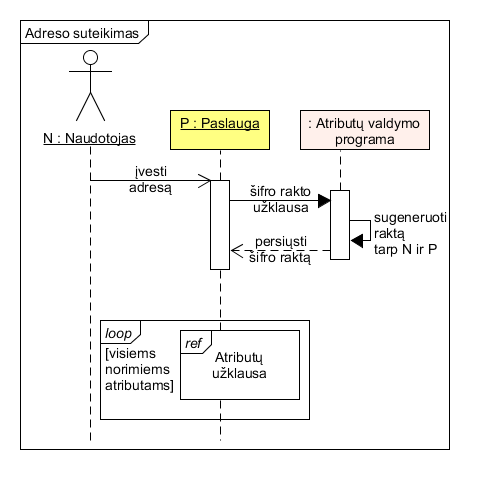
\includegraphics[scale=0.6]{img/userGivesAddress}
    \caption{Naudotojas adreso suteikimas paslaugai}
    \label{fig:userGivesAddress}
\end{figure}

\subsubsection{Paslaugos atliekama atributo užklausa} \label{BCIDM:askForAttribute}

Paslauga P, norinti gauti tam tikrą asmens atributą (pvz. gimimo datą), kreipiasi į blokų grandinės išmanųjį kontraktą (žr.~\ref{fig:askForAttributeSequence} pav.).
Kontraktas tuomet patikrina, ar ši paslauga turi prieigą prie pageidaujamo atributo. Jei turi, tuomet grąžina šį atributą. Jis
užšifruotas paslaugos P turimu šifro raktu, tad paslauga gali jį dešifruoti ir perskaityti duomenis. Jei
naudotojas atmetęs prieigą, apie tai pranešama paslaugai. Jei naudotojas dar nesvarstęs šios prieigos, išsaugoma laukianti
(angl. \textit{pending}) paslaugos P atributo A užklausa ir laukiama naudotojo sprendimo. Naudotojas šią laukiančią užklausą galės pamatyti savo 
atributų valdymo programoje ir ten atlikti sprendimą.

\begin{figure}[h]
    \centering
    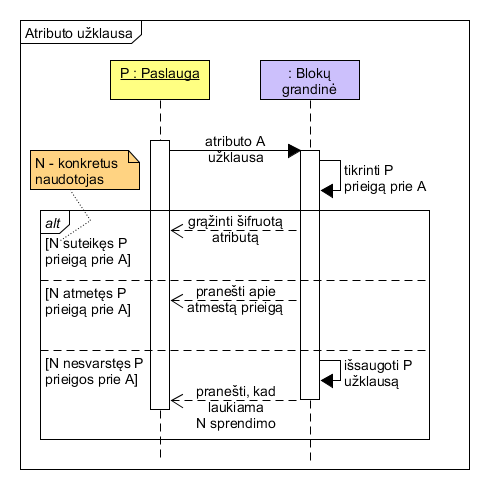
\includegraphics[scale=0.7]{img/askForAttributeSequence}
    \caption{Pirmas naudotojo pasinaudojimas paslauga}
    \label{fig:askForAttributeSequence}
\end{figure}

\subsubsection{Naudotojo atliekamas paslaugos autorizavimas}

atributų valdymo programa, stebinti išmaniuosiuose kontraktuose naujas paslaugų užklausas, praneša naudotojui apie dar
neatliktus autorizavimus. Tuomet naudotojas gali pasirinkti, ar suteikti, ar atmesti prieigą prie norimo atributo
A paslaugai P. (žr.~\ref{fig:givePermissions} pav.)\\
Jei naudotojas prieigą suteikia, tuomet atributų valdymo programa prašo pasirinkti, iš kur naudoti duomenis atributui. Tai
daroma todėl, kad kiekvienas atributas, suteiktas paslaugai P, turi būti užšifruotas tik paslaugai P ir naudotojui N
žinomu šifro raktu bei nusiųstas
į išmanųjį kontraktą. Pasirinkus, kokius duomenis šifruoti (naudotojas galėtų juos įvesti pats arba pasirinkti, kad
jie būtų imami iš tapatybės tiekėjo), jie nusiunčiami į išmanųjį kontraktą ir jame pažymima, kad paslauga P autorizuota
pasiekti atributą A.\\
Jei naudotojas prieigą atmeta, tuomet blokų grandinėje pažymima, kad paslauga P nėra autorizuota pasiekti atributą A.

Jei naudotojas vėliau nuspręstų pakeisti savo sprendimą (pvz. panaikinti suteiktas prieigas prie atributo A paslaugai P),
jis šį paslaugos autorizavimo procesą galėtų pakartoti ir jau esamai prieigai.


\begin{figure}[h]
    \centering
    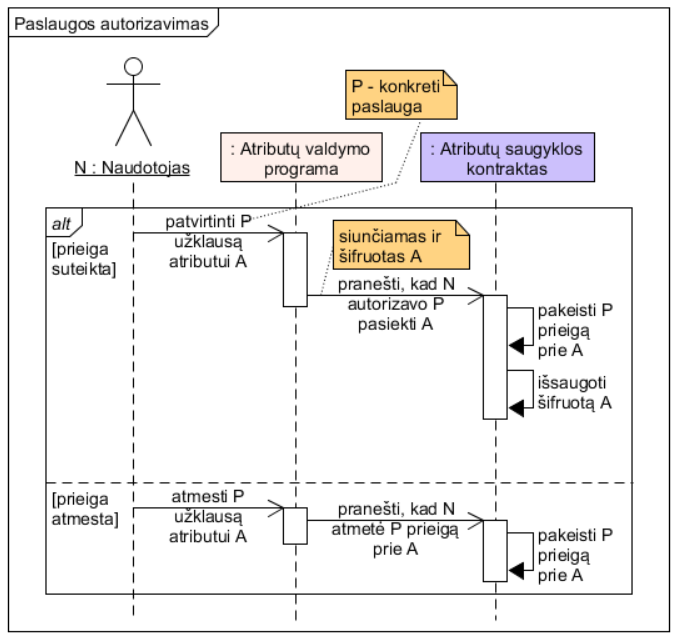
\includegraphics[scale=0.65]{img/givePermissions}
    \caption{Pirmas naudotojo pasinaudojimas paslauga}
    \label{fig:givePermissions}
\end{figure}

\subsubsection{Atributų valdymo programos atliekamas blokų grandinės stebėjimas} \label{BCIDM:blockchainMonitoring}

Blokų grandinės išmanusis kontraktas negali tiesiogiai pranešti išorinei (ne išmaniajame kontrakte esančiai) programai
apie įvykusius pasikeitimus. Todėl išmanusis kontraktas gali saugoti būseną, o ją vėliau pasiekia norinti taikomoji programa.
Tokiu būdu atributų valdymo programa periodiškai kreipiasi į išmanųjį kontraktą ir žiūri, ar yra naujų paslaugų užklausų. Jeigu jų yra,
atributų valdymo programa išsaugo pranešimą apie tai naudotojui (žr.~\ref{fig:checkForPendingPermissions} pav.).\\
Panašiu stebėjimo principu pasikeitimus išmaniojo kontrakto būsenoje gali stebėti ir paslaugų tiekėjai
(pvz. apie pasikeitusias prieigas).

\begin{figure}[h]
    \centering
    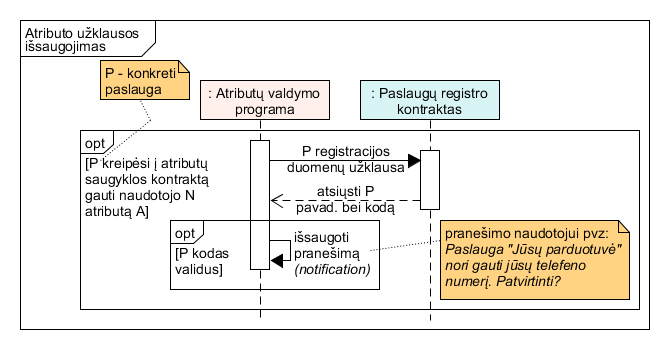
\includegraphics[scale=0.6]{img/checkForPendingPermissions}
    \caption{Pirmas naudotojo pasinaudojimas paslauga}
    \label{fig:checkForPendingPermissions}
\end{figure}

\subsection{Paslaugų atpažinimas iš adreso}

Šiame modelyje paslaugos yra identifikuojamos pagal jų blokų grandinės paskyros adresą. Atributų valdymo programa,
skaitanti išmaniajame kontrakte laukiančias užklausas, jose mato išsaugotą besikreipusios paslaugos adresą.

Nors adresas yra viešas ir unikaliai identifikuoja kiekvieną blokų grandinės dalyvį, turintį paskyrą, tačiau iš adreso nustatyti tikrąją dalyvio tapatybę yra sudėtinga -
pats adresas nėra tiesiogiai susiejamas su tikru asmens identifikatoriumi (pvz. asmens kodu ar paslaugos įmonės kodu).
Tokiu būdu, atributų valdymo programoje matant tik paslaugos adresą dalyvis gali nežinoti, kokią paslaugą jis autorizuoja.

Sprendimas panaikinti šį anonimiškumą būtų sukurti išmanųjį kontraktą, kuris funkcionuotų kaip \textit{paslaugų registras}. Kiekviena
paslauga turėtų atlikti vieną transakciją į šį registrą, nusiunčiant savo vardą ir taip kontraktas išsaugotų, iš kokio adreso į jį kreiptąsi (nes
transakcija yra pasirašyta kontrakto kvietėjo ir tik jis gali atlikti transakcijos iš jo paskyros). Tuomet, paslaugai viešai
atskleidus savo adresą (pvz. pateikus savo tinklalapyje prieigos tašką (angl. \textit{endpoint}), kuris jį grąžina), būtų galima
nesunkiai patikrinti, ar paslauga, besiskelbianti adresu X, iš tikrųjų yra užsiregistravusi \textit{paslaugų registre}. Tokiu būdu
atributų valdymo programa galėtų kreiptis į \textit{paslaugų registrą}, patikrinti ar paslauga jame yra ir iš jo sužinoti paslaugos
pavadinimą. 
\section{Tapatybės atributų valdymo modelio prototipas}

Tapatybės atributų valdymo modelis sudarytas iš 3 dalių: atributų saugyklos kontrakto, paslaugų registro kontrakto bei
atributų valdymo programos (žr. \hypertarget{BCIDM:blockchainFunctions}{\ref{BCIDM:blockchainFunctions}} sk.).
Siekiant patvirtinti galimą modelio veikimą, \enquote{Solidity} programavimo kalba \enquote{Ethereum} blokų grandinei
realizuoti atributų saugyklos bei paslaugų registrų kontraktai. 

\subsection{Pasirinktos technologijos}

Išmaniesiems kontraktams programuoti pasirinkta naudoti \enquote{Ethereum} platformą ir \enquote{Solidity} programavimo
kalbą. Priežastys tam:

\begin{itemize}
    \item programuotojų bendruomenė. Nuo 2015-ųjų veikianti \enquote{Ethereum} platforma turi nemažą
    palaikančių asmenų bendruomenę, kuri prisideda prie pačio \enquote{Ethereum} atviro kodo vystymo
    bei atsako į pradedančiųjų klausimus;
    \item technologijos branda. Kai išmaniųjų kontraktų programavimas yra vis dar gana nauja sritis,
    \enquote{Ethereum} technologija, veikianti nuo 2015-ųjų, yra gana gerai dokumentuota, o rekomenduojama kontraktams rašyti programavimo kalba
    \enquote{Solidity} \cite{Ethereum} turi keletą skirtingų kūrimo karkasų programavimo aplinkai paruošti \cite{SolidityDocumentation}.
\end{itemize}

Išmanieji kontraktai kurti naudojant \enquote{Solidity} programavimui skirtą \enquote{Truffle} kūrimo karkasą,
taikant \enquote{ganache-cli} lokalią blokų grandinę testavimui. Kontraktų funkcijos išbandytos jas kviečiant iš sukurto testinio
\enquote{React} puslapio. Kodas pasiekiamas \enquote{GitHub} repozitorijoje
\url{https://github.com/Ubaldas11/blockchain-attribute-management}.

Išmaniosios programėlės maketai kurti su X prototipavimo įrankiu.

\subsection{Atributų saugyklos kontraktas}

Kontraktas skirtas naudotojų atributų saugojimui bei prieigų suteikimui realizuoti. Kontraktas sudarytas iš kontrakto saugyklos,
kurioje saugomos koduotos atributų reikšmės ir jų prieigos, įvykių bei funkcijų.
Kontrakto kodas pateikiamas priede \hypertarget{appendix:attributeSmartContract}{\ref{appendix:attributeSmartContract}}.

Kontrakte apibrėžti šie įvykiai:

\begin{enumerate}
    \item \textit{AccessRequested}. Skirtas pranešti, kad paslauga P prašo prieigos prie naudotojo N atributo A. Šio įvykio laukia
    atributų valdymo programa ir jį gavusi, gali pranešti naudotojui N apie naują paslaugos P užklausą.
    \item \textit{AccessChanged}. Skirtas pranešti, kad naudotojas N pakeitė paslaugos P prieigą prie atributo A. Paslaugos, 
    laukiančios šio įvykio, jį gavusios sužino apie galimai suteiktą arba panaikintą prieigą prie atributo A.
\end{enumerate}

Kontrakte apibrėžtos šios viešos funkcijos:

\begin{enumerate}
    \item \textit{grantAccess}. Skirta naudotojui N suteikti paslaugai P prieigą prie atributo A. Į funkciją paduodamas A identifikatorius,
    P adresas bei N ir P šifro raktu užkoduota A reikšmė. Funkcijoje keičiama siuntėjo atributo reikšmė - taip užtikrinama, kad naudotojas N
    negalės pakeisti naudotojo N1 atributo. Funkcija paskelbia \textit{AccessChanged} įvykį;
    \item \textit{removeAccess}. Skirta naudotojui N panaikinti paslaugos P prieigą prie atributo A. Į funkciją paduodamas A identifikatorius ir P
    adresas. Kaip ir \textit{grantAccess} atveju, keičiama siuntėjo atributo prieiga. Funkcija paskelbia \textit{AccessChanged} įvykį;
    \item \textit{requestAccess}. Skirta paslaugai P pranešti, kad ji nori prieigos prie naudotojo N atributo A reikšmės. Į funkciją paduodamas A identifikatorius
    bei N adresas. Funkcija paskelbia \textit{AccessRequested} įvykį;
    \item \textit{getAttribute}. Skirta gauti naudotojo N paslaugai P skirtą atributą A. Į funkciją paduodamas A identifikatorius, N adresas bei
    P adresas. Jei funkciją iškvietė N (t.y., pats naudotojas kreipiasi gauti suteiktą atributą A), grąžinamas siekiamas atributas. Jei kreipiasi paslauga,
    galimos 3 grąžinamos reikšmės. Jei prieiga naudotojo suteikta - grąžinama A reikšmė. Jei prieiga atmesta - pranešama, kad paslauga neautorizuota. Jei
    prieiga naudotojo dar nebuvo svarstyta, prašoma pirma kreiptis į \textit{requestAttributeAccess} funkciją.\\
    Funkcija realizuota kaip vaizdo (angl. \textit{view}) funkcija - ji nekeičia kontrakto būsenos, todėl jos kvietimas yra nemokamas.
\end{enumerate}

Kadangi įvykių paskelbimas yra pigesnis nei kontrakto būsenos keitimas, tai išnaudota paskelbiant apie naują prieigos užklausą (vietoj alternatyvos pakeisti
kontrakto būseną ir nurodyti, kad paslauga kreipėsi). Jei paslauga arba atributų valdymo programa realiu laiku \enquote{neišgirdo} įvykio, ji vėliau gali
pasiekti visą įvykių sąrašą (angl. \textit{log)}.

\subsection{Paslaugų registro kontraktas}

Kontraktas skirtas užsiregistravusių paslaugų sąrašui saugoti. Paslaugų siųstuose įrašuose laikomas
registracijos kodas bei paslaugos pavadinimas.
Kontrakto kodas pateikiamas priede\hypertarget{appendix:serviceRegisterContract}{~\ref{appendix:serviceRegisterContract}}.

Kontraktą sudaro dvi funkcijos:

\begin{enumerate}
    \item \textit{register}. Skirta paslaugai užsiregistruoti. Į funkciją paduodamas registracijos kodas bei paslaugos pavadinimas, kurie išsaugomi kontrakto būsenoje.
    \item \textit{getService}. Skirta atributų valdymo programai išgauti duomenis apie besikreipusią paslaugą. Funkcijai paduodamas paslaugos adresas.
    Funkcija realizuota kaip vaizdo (angl. \textit{view}) funkcija - ji nekeičia kontrakto būsenos, todėl jos kvietimas yra nemokamas. \\ 
    Atributų valdymo programa kreipiasi į šią funkciją tuomet, kai gauta nauja paslaugos P atributo A užklausa.
    Iš gauto kodo programa gali atskirti, ar ši paslauga nėra apsimetelė
    (žr.\hypertarget{BCIDM:serviceRegister}{~\ref{BCIDM:serviceRegister} skyrelį}). Jei kodas nesutampa, atributo prieigos užklausą galima ignoruoti. Jei kodas sutampa,
    gautą pavadinimą galima rodyti atributų valdymo programoje ir pranešti apie prieigos užklausą naudotojui.
\end{enumerate}
\section{Tapatybės atributų valdymo modelio vertinimas} \label{section:blockchainIDMevaluation}

Šiame skyriuje vertinamas\hypertarget{section:BCIDM}{~\ref{section:BCIDM}} skyriuje pristatytas blokų grandine paremtas tapatybės atributų
valdymo modelis: kokie jo privalumai, trūkumai, pritaikymo barjerai.

\subsection{Privalumai}

\subsubsection{Naudotojui suteikta atributų valdymo kontrolė}

Naudotojas su atributų valdymo programa gali autorizuoti paslaugas pasiekti jo atributus, esančius blokų grandinėje. Programoje
taip pat galima pamatyti visus įvestus atributus ir paslaugas, kurios yra autorizuotos juos pasiekti. Naudotojas taip pat
gali pakeisti anksčiau priimtą sprendimą ir programa atnaujins prieigą blokų grandinėje. Naudotojui nusprendus pakeisti
atributo reikšmę, jis tai padaro atributų valdymo programoje, o ši kreipiasi į blokų grandinę ir joje atnaujina esančias reikšmes. Kaip
galėtų atrodyti tokia atributų valdymo programa pateikiama priede\hypertarget{appendix:attributeManagementApp}{~\ref{appendix:attributeManagementApp}}.\\
Išvardytos funkcijos padengia\hypertarget{BCIDM:requirements}{~\ref{BCIDM:requirements}} skyrelio 1, 2 ir 3 reikalavimus.

\subsubsection{Decentralizuoti asmens duomenys}

Tapatybės duomenis saugant blokų grandinėje, atributai tampa pasiekiami nepriklausomai nuo vienos trečiosios šalies pasiekiamumo.
Taip tiek paslaugų tiekėjai, tiek naudotojas gali betkada pamatyti suteiktus atributus tol, kol bent vienas blokų grandinės mazgas
yra pasiekiamas. Taip pat, nors duomenys decentralizuoti, dėl jų šifravimo jie išlieka prieinami tik naudotojui ir jo pasirinktoms
paslaugoms.
Šis privalumas įgyvendina\hypertarget{BCIDM:requirements}{~\ref{BCIDM:requirements}} skyrelio 4-ą reikalavimą.

\subsubsection{Sumažintas reikalingas pasitikėjimas trečiosiomis šalimis}

Kadangi tapatybės atributai yra saugomi viešoje, decentralizuotoje blokų grandinėje, kurios išmaniųjų kontraktų
logika prieinama visiems, naudotojams nebereikia pasitikėti vien tik paslaugų bei tapatybės tiekėjais - jų
atributai šiuo atveju priklauso nuo korektiško išmaniųjų kontraktų veikimo.

Verta pastebėti, kad
pristatytame modelyje naudotojui vis dar reikia pasitikėti atributų valdymo programos veikimu. Tačiau, ši programa pati
asmens duomenų nesaugo (tik persiunčia įvestas ir grąžina blokų grandinėje esančias reikšmes). Pasitikėjimui
padidinti ši programa taip pat turėtų būti viešai prieinamo atviro kodo.

Taip pat, paslaugų tiekėjai, parsisiuntę atributą
iš blokų grandinės, vis dar gali jį išsisaugoti. Tačiau, galimybė paslaugai pačiai nesaugoti naudotojo duomenų turėtų būti pagrindinė paskata
naudotis šiuo modeliu - taip naudotojai labiau pasitikės šia paslauga. Galimas išsisaugojimo pavojus pastebimas ir
\cite{MITPaper} tyrime, kurio autoriai aptaria ir galimybę neleisti paslaugai pasiekti pačio duomens, o atlikti
reikalingus skaičiavimus pačiame blokų grandinės tinkle.

\subsection{Trūkumai}

\subsubsection{Paslaugų autentiškumo tikrinimas}

Modelyje aprašytas paslaugų registras padeda apsisaugoti nuo programišių, galinčių apsimesti paslaugomis. Šio registro veikimas
nėra itin patogus, nes kiekviena paslauga turi gauti sugeneruotą kodą iš atributų valdymo programos ir įrašyti jį į atskirą išmanųjį kontraktą.
Tai reikalauja daugiau integracijų (tarp paslaugos, atributų valdymo programos ir papildomo išmaniojo kontrakto)
bei papildomo naudotojo pasitikėjimo atributų valdymo programa: jai patikėta generuoti kodą bei atlikti paslaugos registracijos
tikrinimą.

Galimos kelios alternatyvos paslaugų identifikavimui užtikrinti. Galima būtų naudotis jau egzistuojančiais identiteto
registravimo projektais, kuriuose paslaugos užregistruotų savo tapatybę (pvz. \enquote{NameCoin} ar \hypertarget{section:relatedWork}{\ref{section:relatedWork}}
skyrelyje minimu \enquote{Blockstack}). Kitas būdas, aptariamas \cite{Baars2016} tyrime, būtų turėti registrą, kuriame paslaugų autentiškumą
patvirtintų patikima trečioji šalis (pvz. bankas ar valdžios įstaiga). Tokiu atveju, paslaugos turėtų autentifikuotis šios institucijos
sistemoje, o ji įrašytų į paslaugų registrą apie sėkmingą paslaugos registraciją. Tokiu atveju pasitikėjimas būtų perkeliamas
pasirinktoms institucijoms.

\subsubsection{Nepatikimos atributų reikšmės}

Paslaugų tiekėjai iš blokų grandinės gauna reikšmes, kurias įvedė pats naudotojas. Tai nesudaro jokių keblumų,
kai jų teisingumą gali patikrinti pati paslauga (pvz. atsiųsti žinutę į telefono numerį), tačiau kai to atlikti negalima,
paslaugai tenka pasitikėti naudotojo įvesta reikšme.

Tai būtų galima tobulinti, jei šias reikšmes galėtų verifikuoti
atsakingos institucijos (pvz. bankas). Tuomet, šios institucijos turėtų teikti papildomą paslaugą, kurioje naudotojui
paprašius, jos galėtų atlikti užklausą į blokų grandinę ir patvirtinti, kad atributo reikšmė yra teisinga, o tai būtų
išsaugota išmaniajame kontrakte. Tokiu atveju,
į blokų grandinę besikreipianti paslauga galėtų matyti, ar šis atributas yra verifikuotas. Panašus tvirtinimo mechanizmas
nagrinėjamas \cite{Baars2016} tyrime.

\subsubsection{Kaina}

Blokų grandinės išmaniųjų kontraktų funkcijų kvietimai kainuoja pinigus. Pagal nutylėjimą, už funkcijos kvietimą sumoką kvietėjas.
Naudojant \hypertarget{tab:contractPrices}{\ref{tab:contractPrices}} lentelėje pateiktas kainas, galima įvertinti
preliminarią modelio naudojimo kainą \enquote{Ethereum} blokų grandinėje.
Vienkartinis kontraktų sukūrimo mokestis: 5,76€ (3,72 + 2,04). Daromos modelio naudojimo prielaidos:

\begin{itemize}
    \item naudotojas per mėnesį pradeda naudotis 3-imis naujomis paslaugomis,
    \item naudotojas per mėnesį atmeta 5-ias paslaugų atributų užklausas,
    \item naudotojas per mėnesį pakeičia 3-is paslaugų prieigas,
    \item naudotojas per mėnesį pakeičia 1-o atributo reikšmę,
    \item paslaugai vidutiniškai reikia 5-ių atributų reikšmių,
    \item paslauga per mėnesį įgauna 500 naujų naudotojų.
\end{itemize}

Tuomet mėnesinė kaina naudotojui: 6,5€ (3*5*0,25 + 5*0,25 + 5*0,25 + 1*0,25). Mėnesinė kaina paslaugai: 300€ (500*5*0,12).
Kai naudotojas gali būti linkęs mokėti mėnesinį mokestį už didesnę tapatybės atributų kontrolę ir decentralizuotus asmens duomenis,
išlieka klausimas, ar paslaugos tiekėjas sutiks mokėti naudojimosi kainą už jo naudotojams suteiktą didesnę kontrolę bei pašalintą poreikį
pačiam saugoti atributus.

Vienas iš galimų sprendimų - kviečiant funkciją paslaugai, ją apmokėtų ne paslaugos tiekėjas, o pats išmanusis kontraktas. Kontrakto lėšas
galima būtų pildyti iš mėnesinio naudotojų mokesčio.
Tačiau, tokį mechanizmą turi palaikyti pasirinkta blokų grandinė, taikant jį reiktų apsisaugoti ir nuo
galimų pavojingų pakartotinių kvietimų, kurie būtų skirti tik išeikvoti kontrakto lėšas. Kitas galimas būdas - mažinti saugomų duomenų kiekį
pačioje blokų grandinėje (taip išmaniųjų kontraktų išlaikymo kainos taptų mažesnės) iškeliant atributų reikšmes į šalutinę grandinę (angl. \textit{off-chain}).

\subsection{Pritaikymo barjerai}

Pagrindiniai sunkumai, kurie kiltų tokį modelį taikant praktikoje, yra galimas paslaugų nenoras bendradarbiauti bei menka blokų grandinės
technologijos branda.

Paslaugų tiekėjams, norint pradėti naudoti šį modelį savo paslaugose, reikia susikurti blokų grandinės paskyrą bei suintegruoti
savo sistemas su blokų grandinės išmaniaisiais kontraktais bei atributų valdymo programa.
Tai gali būti palengvinta sukuriant viešai prieinamą programinę įrangą, paruoštą naudoti paslaugų
tiekėjams, tačiau paslaugų kūrėjai vis tiek turi nuspręsti naudoti šį modelį. Pagrindinė paskata jiems yra didesnis naudotojų pasitikėjimas
suteikiant jiems galimybę kontroliuoti savo duomenis bei pagerintas asmens duomenų pasiekiamumas juos iškėlus į decentralizuotą blokų grandinę.

Blokų grandinė yra vis dar gana nauja technologija. Vieša blokų grandinė gali būti pažeista daugumos atakos, nemažai skeptikų
teigia, kad pagrindinis technologijos panaudojimas išliks tik kriptovaliutoms, technologijos plečiamumas (angl. \textit{scalability}) aktyviai
tiriamas. Taip pat, 2016-aisiais metais išmaniojo kontrakto \enquote{The DAO} trūkumą išnaudojusi ataka privertė \enquote{Ethereum} 
blokų grandinę atlikti išsišakojimą (angl. \textit{hard fork}), kuris pakeitė transakcijų istoriją ir grąžino įsilaužėlio
pavogtą kriptovaliutą jos savininkams \cite{TheDAO}. Tai rodo, kad ypatingomis sąlygomis blokų grandinės nekintamumas gali būti pažeistas.

Nepaisant išvardytų priežasčių, technologijos populiarumas neblėsta. Blokų grandinės technologiją pradeda naudoti didžiosios kompanijos
(\enquote{Microsoft} bei \enquote{IBM} siūlo
blokų grandinę kaip paslaugą \cite{Zheng2017}). Taip pat, vis daugiau programuotojų kuria išmaniuosius kontraktus
(darbo rašymo metu \enquote{Ethereum} blokų grandinėje yra 25374 verifikuoti išmanieji kontraktai \cite{EthVerifiedContracts}).

Blokų grandinė dar nėra brandi, ilgai taikoma technologija. Ji aktyviai bandoma tiek startuolių, tiek
korporacijų, vis dar intensyviai tiriama mokslininkų. Technologiją naudojančių programų sėkmė nulems, ar asmenys
sutiks naudotis blokų grandine paremtomis programomis.







\sectionnonum{Rezultatai ir išvados}

Darbe pasiekti \textbf{rezultatai}:

\begin{enumerate}
    \item Apžvelgus internete
    naudojamus skaitmeninės tapatybės valdymo modelius, apibendrintos esminės naudotojams kylančios problemos: nepakankama asmens duomenų
    kontrolė, mažėjantis pasitikėjimas paslaugų gebėjimu saugiai valdyti asmens duomenis, didelė priklausomybė nuo tapatybės tiekėjų.
    \item Pristačius blokų grandinės technologiją ir ją naudojančius skaitmeninės tapatybės projektus, nustatyta, kad decentralizuotas
    asmens duomenų saugojimas bei duomenų suteikimo taisyklių aprašymas išmaniuosiuose kontraktuose
    suteikia pagrindo naudoti blokų grandinę skaitmeninės tapatybės atributų valdymui.
    \item Parengti reikalavimai skaitmeninės tapatybės atributų valdymo modeliui, akcentuojantys įvardytas naudotojų problemas.
    \item Pagal iškeltus reikalavimus paruoštas blokų grandine paremtas tapatybės atributų valdymo modelis, suteikiantis naudotojui galimybę kontroliuoti savo asmens duomenis
    bei autorizuoti paslaugų prieigą prie jų.
    \item Realizuoti pristatyto modelio atributų saugyklos bei paslaugų registro išmanieji kontraktai, parašyti \enquote{Solidity} programavimo kalba \enquote{Ethereum} blokų grandinei.
    Sukurtas atributų valdymo mobiliosios programėlės interaktyvus prototipas.
    \item Įvertintas pristatytas atributų valdymo modelis. Įvardyti jo privalumai, trūkumai,
    galima eksploatavimo kaina bei pritaikymo barjerai.
\end{enumerate}

\hfill \break
Išanalizavus rezultatus gautos darbo \textbf{išvados}:

\renewcommand{\labelenumii}{\arabic{enumii}.}
\begin{enumerate}
    \item Blokų grandinės naudojimas tapatybės atributų valdyme suteikia šiuos pranašumus:
    \begin{enumerate}
        \item Decentralizuotai saugant asmens duomenis,
        panaikinama priklausomybė nuo tapatybės tiekėjo.
        \item Viešuose, visiems prieinamuose
        išmaniuosiuose kontraktuose aprašius paslaugų autorizavimo logiką, naudotojas gali įsitikinti,
        kad jis geba kontroliuoti paslaugų turimas prieigas prie jo asmens duomenų.
        \item Dėl blokų grandinės įrašų ir išmaniųjų kontraktų kodo
        nekintamumo, asmuo gali būti tikras, kad laikui bėgant sąlygos nepasikeis ir naudotojo priimti
        autorizavimo sprendimai išliks.
    \end{enumerate}
    \item Blokų grandinės naudojimas tapatybės atributų valdyme turi šiuos trūkumus:
    \begin{enumerate}
        \item Decentralizuotas kodo vykdymas ir duomenų saugojimas išmaniuosiuose kontraktuose yra gana brangus.
        \item Norint naudotis modeliu, paslaugų tiekėjai yra priversti turėti papildomą integraciją su blokų grandine.
        \item Įmanoma viešos blokų grandinės tinklo daugumos ataka gali atgrasyti potencialius naudotojus.
    \end{enumerate}
    \item Įvertinus nustatytus pranašumus bei trūkumus, galima teigti, kad blokų grandinę skaitmeninės tapatybės atributų valdymui verta naudoti
    tiems naudotojams, kuriems yra itin svarbi jų asmens duomenų kontrolė internete. Plačiau taikyti modelį vertėtų
    sumažinus eksploatavimo kainą bei patobulinus paslaugų atpažinimo procesą.
\end{enumerate}

\hfill \break
Tolimesni galimi darbai:

\begin{enumerate}
    \item Siekiant sumažinti modelio eksploatavimo kainą, ištirti alternatyvas duomenų saugojimui ne blokų grandinėje. Pačioje grandinėje
    paliekant tik nuorodą į duomenų saugojimo vietą, modelio naudojimas taptų pigesnis.
    \item Analizuoti paslaugų identifikavimo alternatyvas. Dabartinis būdas modelyje naudoti paslaugų registrą verčia paslaugų tiekėjus atlikti
    papildomą žingsnį. Taip pat, naudotojas turi pasikliauti atributų valdymo programos atliekamu paslaugos atpažinimu bei registracijos kodo generavimu.
    \item Ištirti paslaugų tiekėjų galimybes naudoti modelį. Supažindinus paslaugų tiekėjus su atributų valdymo modeliu,
    atsižvelgti į jų nuomonę apie galimą naudojimą bei siūlomus patobulinimus.
\end{enumerate}

\printbibliography[heading=bibintoc]
 
\sectionnonum{Sąvokų apibrėžimai}
\textbf{Atributas} - charakteristika, susieta su esybe, pavyzdžiui fiziniu asmeniu. Galimi asmens atributai: gimimo data,
vardas, ūgis, pirštų antspaudai \cite{Camp2004}. Atributas gali būti laikinas (pvz. adresas) arba nuolatinis (pvz. asmens kodas).

\textbf{Identifikatorius} - tai atributas, kuris vienareikšmiškai susiejamas su jį pateikiančiu asmeniu ir kurį
sunku arba neįmanoma pakeisti. Fizinio asmens identifikatoriaus pavyzdys galėtų būti gimimo data
(žmogus gali apie ją meluoti, tačiau gimimo datos pakeisti neįmanoma) \cite{Camp2004}. Skaitmeninio identifikatoriaus
pavyzdys yra naudotojo elektroninio pašto adresas.

\textbf{Identifikavimas} - tai procesas, kurio metu asmuo susiejamas su jo identifikatoriumi \cite{Camp2004}. Identifikavimo
pavyzdys yra asmens ir jo vardo susiejimas: \textit{tu esi Jonas Jonaitis}.

\textbf{Autentifikavimas} - tai procesas, kurio metu patvirtinama sąsaja tarp tapatybės ir jos identifikatoriaus (t.y., įrodoma,
kad asmuo iš tikrųjų yra tas, kas sakosi esąs) \cite{Camp2004, Strictest2011}. Dažniausiai internete autentifikavimui pateikiamas identifikatorius
(pvz. slapyvardis) bei slaptažodis, susietas su tuo identifikatoriumi. Autentifikavimo pavyzdys:
\textit{tavo pateikta slapyvardžio ir slaptažodžio pora patvirtina, kad tu esi Jonas Jonaitis}.

\textbf{Autorizavimas} - tai procesas, kurio metu leidžiama arba draudžiama asmeniui atlikti konkretų veiksmą, priklausomai
nuo jo identifikatoriaus ar atributo \cite{Camp2004}. Pavyzdys: \textit{kadangi tau yra daugiau nei 18 metų, tu gali nusipirkti
energetinį gėrimą}. 

\textbf{Skaitmeninė tapatybė} - abstrakti fizinės esybės reprezentacija, sudaryta iš aibės esybės nuolatinių ar laikinų atributų,
kurie susiejami su fizine esybe \cite{Glasser2009, Camp2004}. Fizinė esybė gali būti fizinis arba juridinis asmuo.
Šiame darbe, jei nenurodyta kitaip, kalbama apie fizinio asmens skaitmeninę tapatybę.

\textbf{Skaitmeninės tapatybės valdymas} (angl. \textit{digital identity management}) - tai veiksmų, skirtų kontroliuoti
tapatybę ir su ja susijusius procesus, visuma \cite{Dabrowski2008}. Į tai įeina autentifikavimas, autorizavimas,
prieigų kontrolė, tapatybės gyvavimo ciklo
valdymas bei saugus tapatybės atributų perdavimas trečiosioms šalims \cite{Cao2010}.

\textbf{Skaitmeninių tapatybių domenas} - tai sritis, kurioje kiekviena tapatybė yra unikali. Domene esantys unikalūs
identifikatoriai leidžia sukurti vienas-su-vienu ryšį tarp šių identifikatorių ir jų tapatybių bei taip vienareikšmiškai
identifikuoti tapatybę iš jos unikalaus identifikatoriaus \cite{Josang2005}.

\textbf{Paslaugų tiekėjas} (angl. \textit{service provider}) - tai betkokia taikomoji programa, kuri suteikia naudotojui tam tikrą paslaugą ar
norimą turinį. Galimi paslaugų tiekėjai yra interneto tinklapiai, susirašinėjimo programos ar kitos taikomosios programos,
į kurias kreipiasi naudotojas \cite{Pashalidis2003, Samar1999}. Paslaugų tiekėjas gali turėti vieną ar kelias paslaugas,
kurioms reikia tapatybės valdymo funkcijų.

\textbf{Tapatybės tiekėjas} (angl. \textit{identity provider}) - servisas ar taikomoji programa, skirta koordinuoti su tapatybe
susijusius duomenis tarp naudotojų, jų naršyklių bei paslaugų tiekėjų \cite{Strictest2011}. Pagrindinės tapatybės tiekėjo funkcijos:
infrastruktūros naudotojų tapatybės duomenims apdoroti sukūrimas ir užklausų iš paslaugų tiekėjų bei naudotojų apdorojimas \cite{Cao2010}.

\textbf{Prieigos raktas} (angl. \textit{token}) - tai objektas, identifikuojantis skaitmeninę tapatybę \cite{TokenDefinition}.
Šis raktas būna išduodamas tapatybės tiekėjo ir skirtas identifikuoti naudotoją. Raktas
būna prisegtas prie visų autentifikuoto naudotojo užklausų ir leidžia paslaugos tiekėjui žinoti, koks naudotojas kreipiasi.

\textbf{Vienkartinis prisijungimas} (angl. \textit{single sign on}) - \textcolor{red}{to be added}.

\appendix
\section{Atributų saugojimo ir autorizavimo kontraktas}
\label{appendix:attributeSmartContract}

\lstinputlisting[language=Java]{annexes/UserAttributeStore.sol}

\section{Paslaugų registro kontraktas}
\label{appendix:serviceRegisterContract}

\lstinputlisting[language=Java]{annexes/ServiceRegister.sol}

\begin{landscape}

\section{Atributų valdymo mobiliosios programėlės interaktyvaus prototipo langai} \label{appendix:appSketches}

\begin{figure}[H]
    \centering
    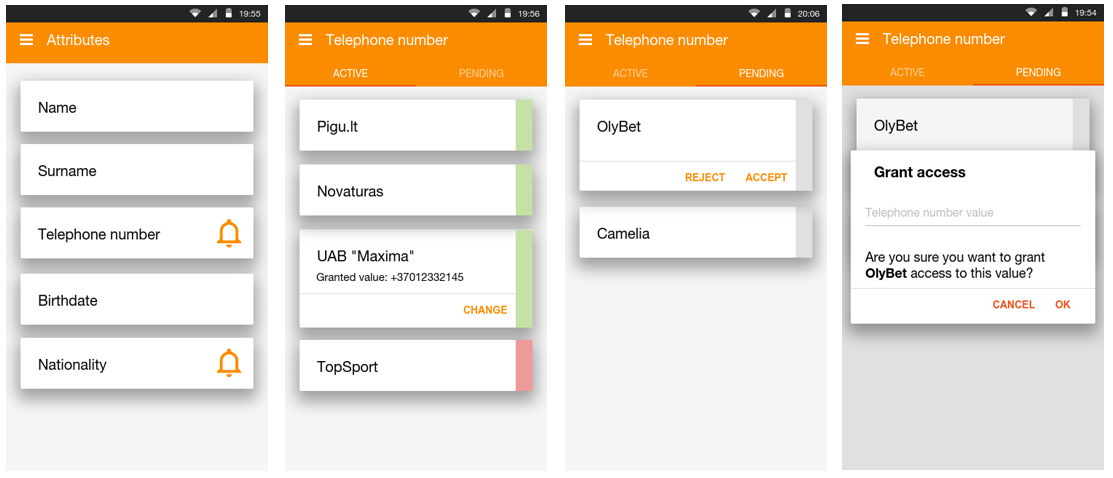
\includegraphics[scale=1]{img/appSketches}
    \caption{Atributų valdymo mobiliosios programėlės interaktyvaus prototipo langai}
    \label{img:appSketches}
\end{figure}

\end{landscape}


\end{document}